\documentclass{article}
\usepackage[utf8]{inputenc}
\usepackage[T1]{fontenc}
\usepackage{amsmath, amssymb}
\usepackage{xcolor}
\usepackage{tikzsymbols}
\usepackage{fontawesome5}
\usepackage[export]{adjustbox}
\usepackage{amssymb}
\usepackage{tikz,lipsum,lmodern}
\usepackage{booktabs}
\usepackage{tikzsymbols}
\usepackage{textcomp}
\usepackage{marvosym}
\usepackage{parskip}
\usepackage{MnSymbol,wasysym}
\usepackage{graphicx}
\usepackage{lipsum}
\usepackage{polynom}
\usepackage{enumitem}
\usepackage{framed}
\usepackage{hyperref}
\usepackage[most]{tcolorbox}
\usepackage{pgfplots}

% Define colors
\definecolor{examplecolor}{RGB}{92, 184, 92}
\definecolor{lessoncolor}{RGB}{74, 144, 226}
\definecolor{notecolor}{RGB}{255, 179, 102}
% Define colors
\definecolor{solutioncolor}{RGB}{74, 144, 226}

% Define new environment for solutions
\newenvironment{solution}{\color{solutioncolor}}{}
% for small text
\newcommand{\smalltext}[1]{\text{\footnotesize #1}}

\title{Advanced Functions Exam - Part C \& D}
\author{Kensukeken}
\date{May 23rd, 2024}

\begin{document}
\maketitle

\subsection*{Part C: Graphing}
1. List the key properties of each graph. Use these to create a sketch. Indicate at least two key points on each curve.
\begin{enumerate}
    \item[a)] \( y = -2x^3 - 6x^2 + 8 \)
    \begin{solution}
           \begin{itemize}
           \item Cubic function with leading coefficient -2, facing downwards.
           \item Key points: \((0, 8)\) (y-intercept), \((-1, 0)\) (crosses x-axis).
       \end{itemize}
     \begin{figure}[h]
    \centering
    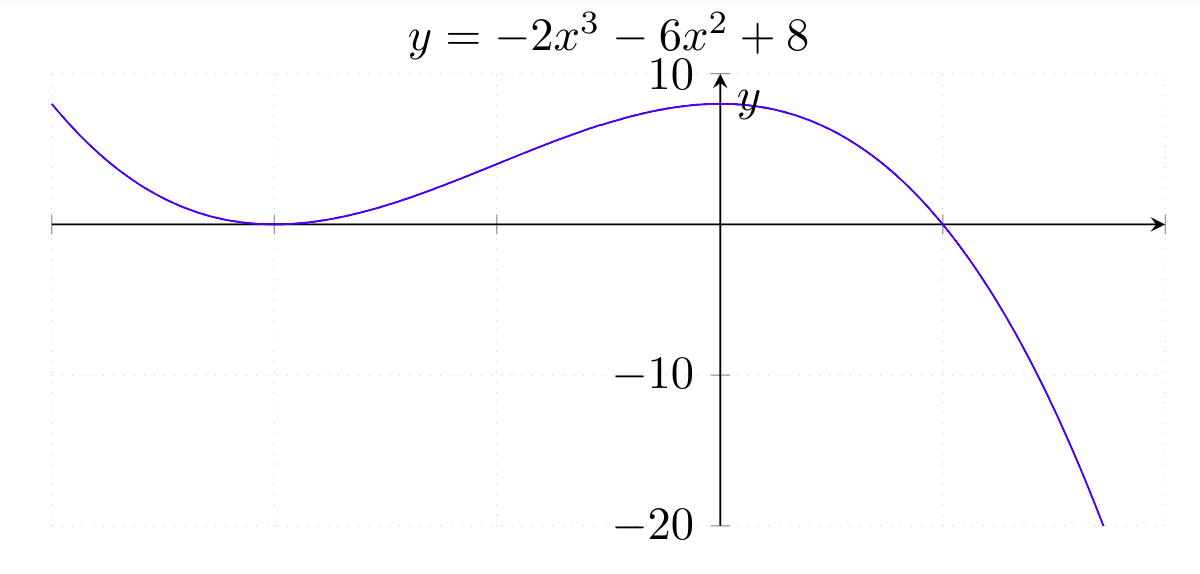
\includegraphics[width=0.62\textwidth]{imgs/imgs FSE/y=-2x^3-6x^2+8.png}
    \label{fig:image}
\end{figure}  
    \end{solution}
%%%%%%%%%%%%%%%%%%%%%%%%%%%%%%%%%%%%%%%%%%%%%%%    
    \item[b)] \( y = \frac{2x + 4}{x - 5} \)
     \begin{solution}  
       \begin{itemize}
           \item Rational function with vertical asymptote at \( x = 5 \).
           \item Key points: \((0, -0.8)\) (y-intercept), \((5, \text{undefined})\) (vertical asymptote).
       \end{itemize}
    \begin{figure}[h]
    \centering
    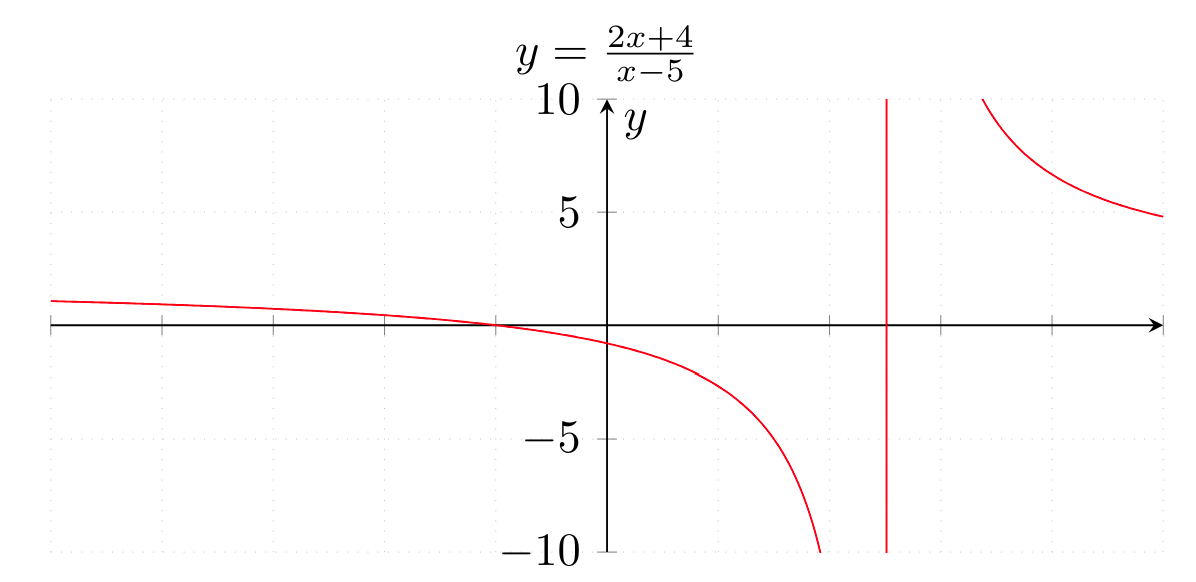
\includegraphics[width=0.62\textwidth]{imgs/imgs FSE/y=2x+4_x-5.png}
    \label{fig:image}
\end{figure}   
    \end{solution}
%%%%%%%%%%%%%%%%%%%%%%%%%%%%%%%%%%%%%%%%%%%%%%%%%%%
    \item[c)] \( y = \frac{1}{x^2 - 4} \)
    \begin{solution}
       \begin{itemize}
           \item Rational function with vertical asymptotes at \( x = \pm 2 \).
           \item Key points: \((0, 0.25)\) (y-intercept), \((2, \text{undefined})\) (vertical asymptote).
       \end{itemize}
     \begin{figure}[h]
    \centering
    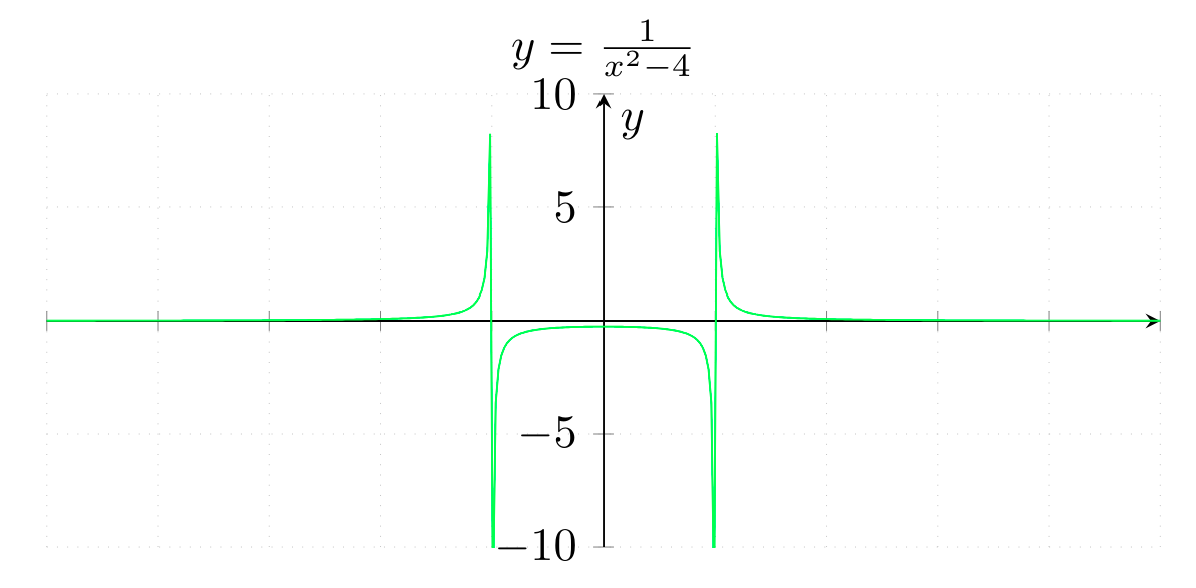
\includegraphics[width=0.62\textwidth]{imgs/imgs FSE/y=1_x^2-4.png}
    \label{fig:image}
\end{figure}  
    \end{solution}
%%%%%%%%%%%%%%%%%%%%%%%%%%%%%%%%%%%%%%%%%%%%%%%%%%%
    \item[e)] \( y = 3\tan(2x - \pi) + 4 \)
    \begin{solution}
       \begin{itemize}
           \item Tangent function with vertical asymptotes.
           \item Key points: \(\left(\frac{\pi}{4}, 4\right)\), \(\left(\frac{3\pi}{4}, 4\right)\).
       \end{itemize}
\begin{figure}[h]
    \centering
    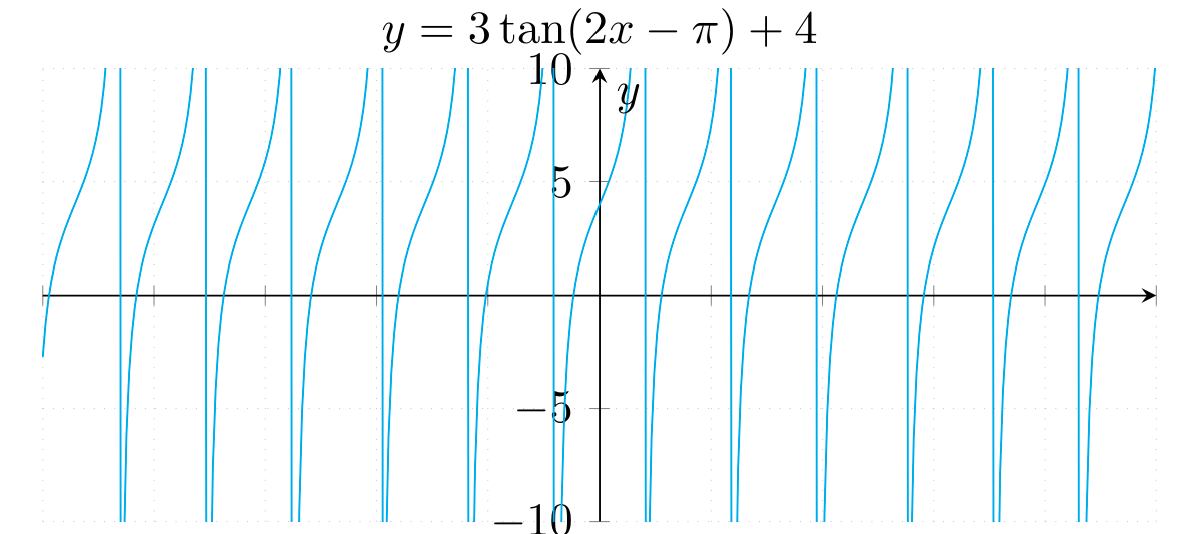
\includegraphics[width=0.62\textwidth]{imgs/imgs FSE/y=3tan(2x-pi)+4.png}
    \label{fig:image}
\end{figure}       
    \end{solution}
%%%%%%%%%%%%%%%%%%%%%%%%%%%%%%%%%%%%%%%%%%%%%%%%%%
    \item[f)] \( y = 2\sec(0.5x) \)
    \begin{solution}
       \begin{itemize}
           \item Secant function with vertical asymptotes.
           \item Key points: \((0, 2)\) (y-intercept), \((4\pi, 2)\).
       \end{itemize}
\begin{figure}[h]
    \centering
    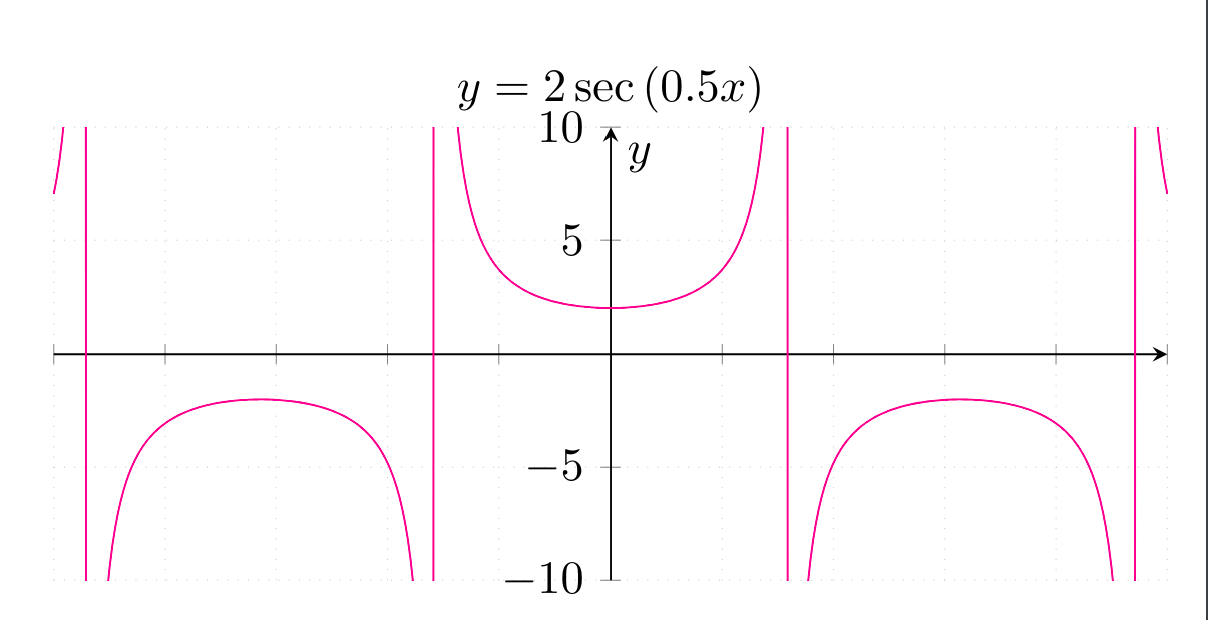
\includegraphics[width=0.62\textwidth]{imgs/imgs FSE/y=2sec(0.5x).png}
    \label{fig:image}
\end{figure}       
    \end{solution}
%%%%%%%%%%%%%%%%%%%%%%%%%%%%%%%%%%%%%%%%%%%%%%%%%%
    \item[g)] \( y = 3^{-x} + 5 \)
    \begin{solution}
       \begin{itemize}
           \item Exponential function approaching \( y = 5 \) as \( x \to \infty \) and \( y = 6 \) as \( x \to -\infty \).
           \item Key points: \((0, 6)\) (y-intercept), \((1, \frac{8}{3})\).
       \end{itemize}
\begin{figure}[h]
    \centering
    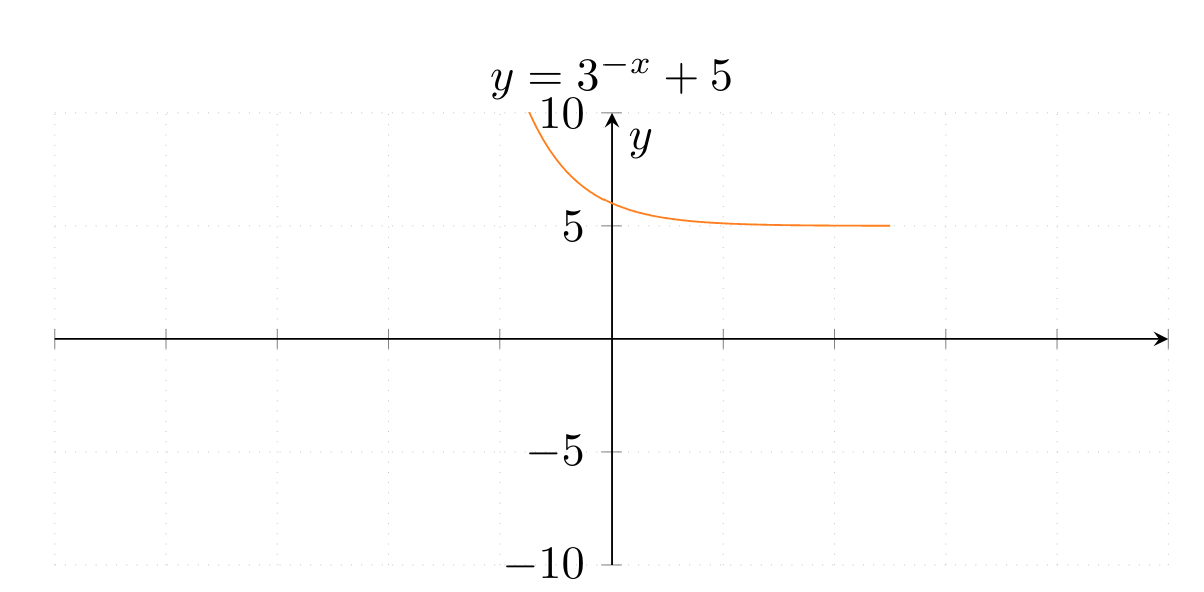
\includegraphics[width=0.62\textwidth]{imgs/imgs FSE/y=3x^-x+5.png}
    \label{fig:image}
\end{figure}       
    \end{solution}
%%%%%%%%%%%%%%%%%%%%%%%%%%%%%%%%%%%%%%%%%%%%%%%    
    \item[h)] \( y = x + \cot(x) \)
    \begin{solution}
       \begin{itemize}
           \item Sum of linear and cotangent functions.
           \item Key points: \((0, 0)\) (origin), \((\pi, \pi)\).
       \end{itemize}
\begin{figure}[h]
    \centering
    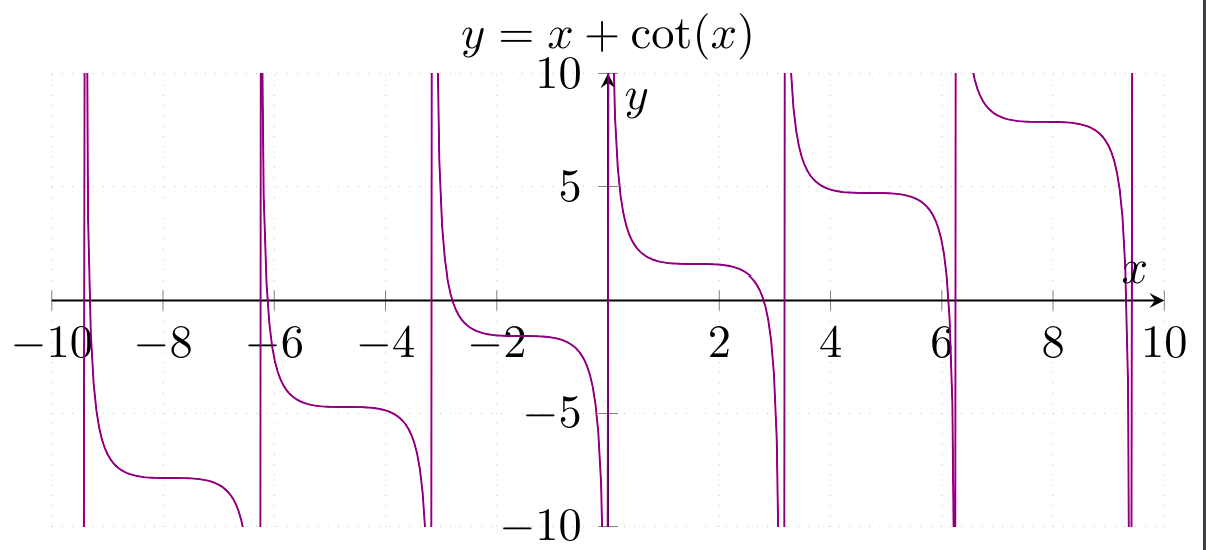
\includegraphics[width=0.62\textwidth]{imgs/imgs FSE/y=x+cotx.png}
    \label{fig:image}
\end{figure}       
    \end{solution}   
\end{enumerate}
%%%%%%%%%%%%%%%%%%%%%%%%%%%%%%%%%%%%%%%%%%%%%%% 

\textbf{Mixed Graphs (All Together)}
\begin{figure}[h]
    \centering
    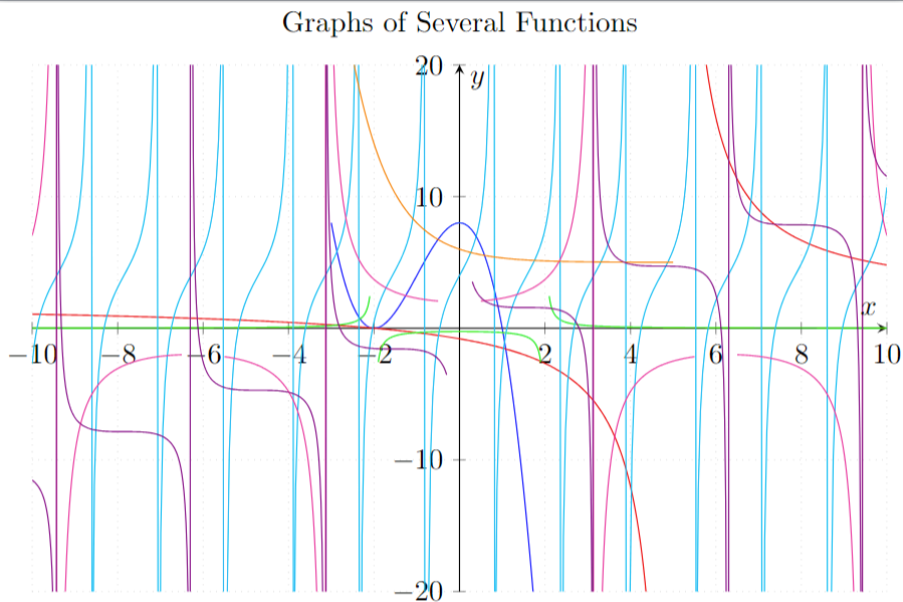
\includegraphics[width=0.62\textwidth]{imgs/imgs FSE/Graph_of_Several_Functions.png}
    \label{fig:image}
\end{figure}   

\newpage

\subsection*{Part D: Reverse Graphing}
1. For each sketch below;
\begin{enumerate}
    \item[a)] List the key properties of the graph.
    \item[b)] What type of relationship is being shown?
    \item[c)] Use a guess and check method to determine the equation of the curve. 
\end{enumerate}


\begin{figure}[h]
    \centering
    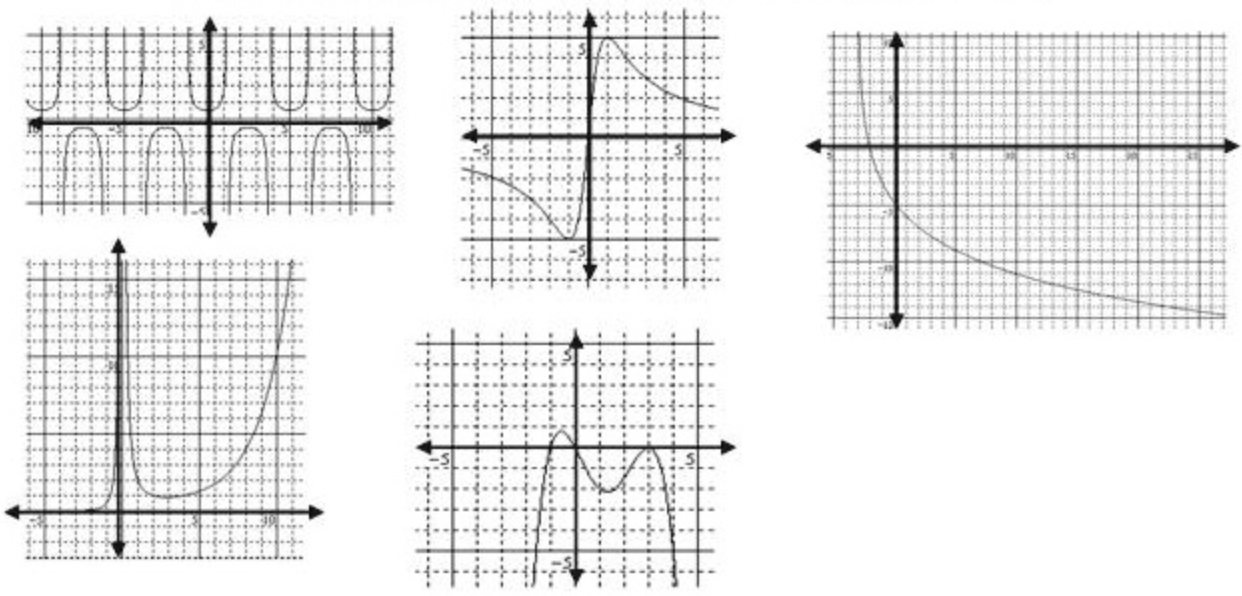
\includegraphics[width=0.9\textwidth]{imgs/imgs FSE/original_graph_part_D.png}
    \caption{Part D: Revere Graphing }
    \label{fig:image}
\end{figure}

\section*{Sources}


Dear Ms. G. Jaksic,

I hope this letter finds you well. I wanted to provide some additional resources regarding the graphs we've been discussing in class. Below, you'll find helpful links that I utilized to create graphs using the \LaTeX \;  typesetting language.

You can access the links here:

\begin{itemize}
    \item \href{https://www.desmos.com/calculator}{Desmos.com.}.
    \item \href{https://www.desmos.com/calculator/funirrjroi}{My work on Desmons.} 
    \item \href{https://www.overleaf.com/read/qnfbffqxnxzc#478dd5}{MHF4U - Advanced Functions Class Notes}
    \item \href{https://www.bu.edu/math/files/2013/08/tikzpgfmanual.pdf}{Learn Tikzpicture here.}
\end{itemize}

Also, I made a graph in Desmos to make sure it's correct. I've attached the pictures for you to see as well.


Thank you for your guidance and support throughout the course. 

Best regards,


Hia Al Saleh


\newpage

\subsection{Graph 1}

% First Graph
\begin{figure}[h]
    \centering
    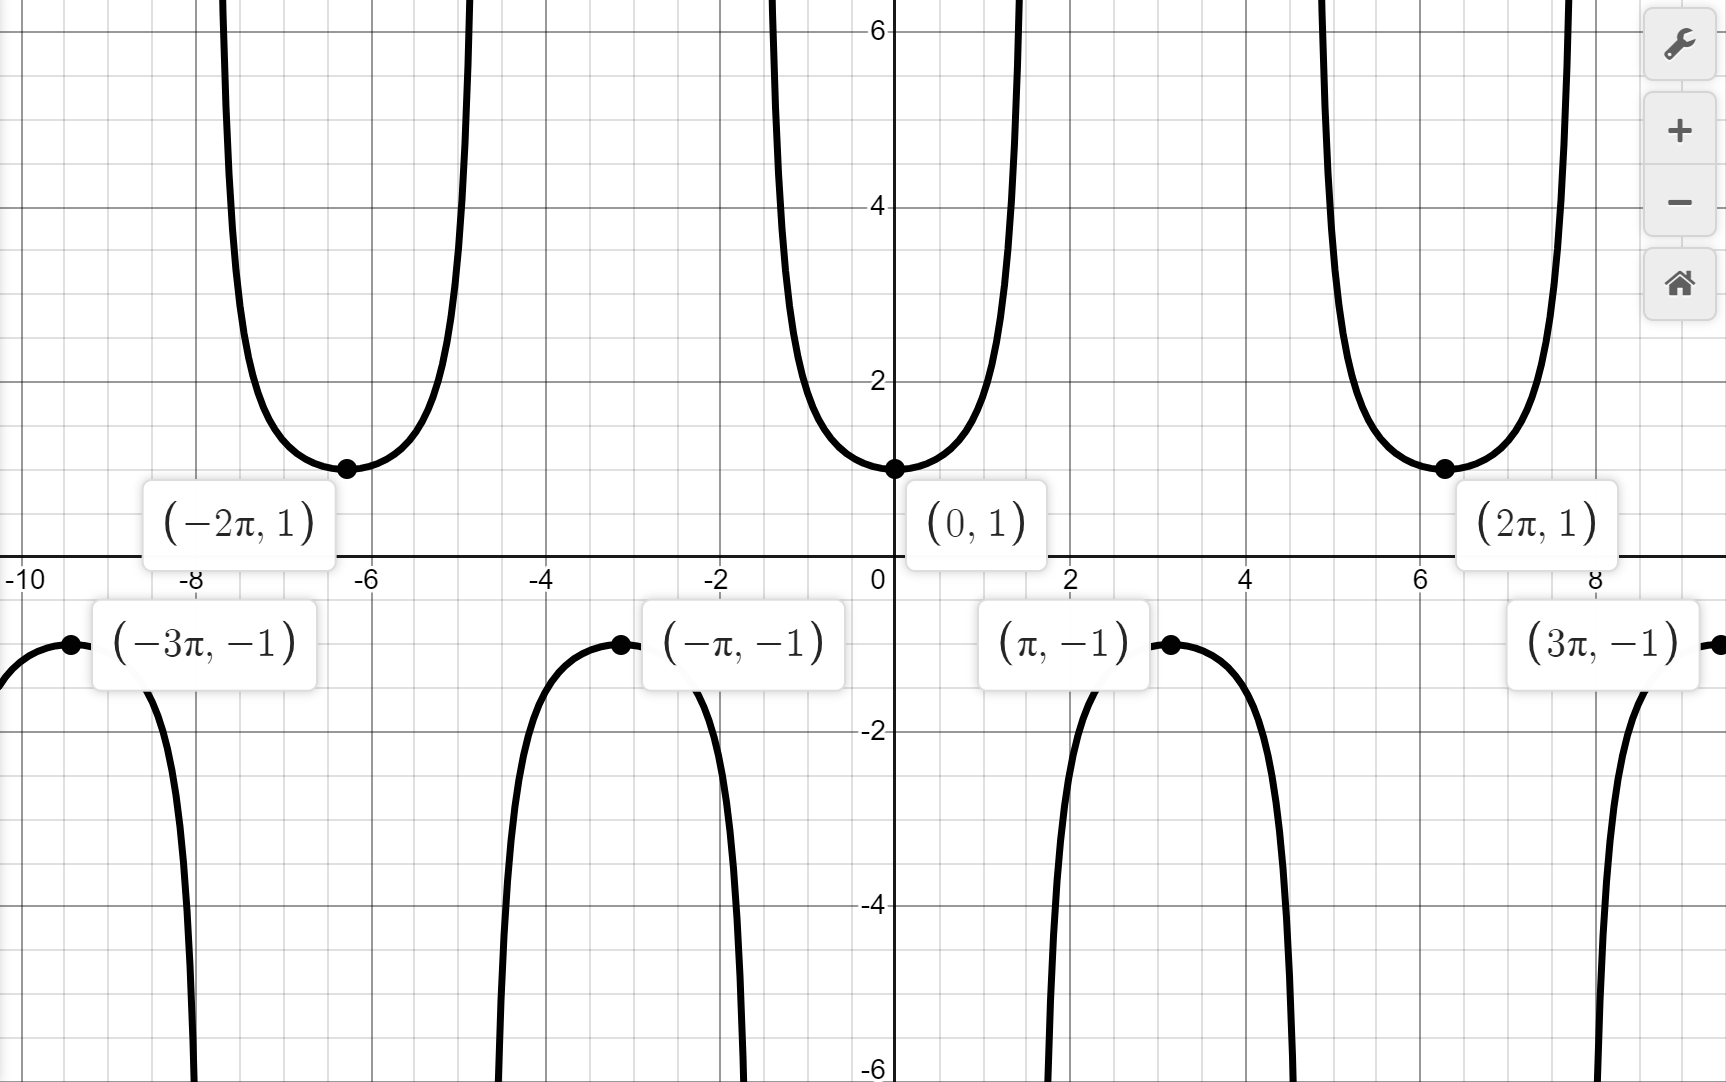
\includegraphics[width=0.9\textwidth]{imgs/imgs FSE/g_1.png}
    \label{fig:image}
\end{figure}
\begin{enumerate}
    \item[a)] \textbf{Key properties:} Periodic function with asymptotes where $\cos x = 0$. 
    \item[b)]  \textbf{Relationship:} Reciprocal of cosine function.
    \item[c)] \textbf{Guess The Equation: } I found my equation for this graph is $$y=\sec x$$
\end{enumerate}
% Equation secx
\begin{figure}[h]
    \centering
    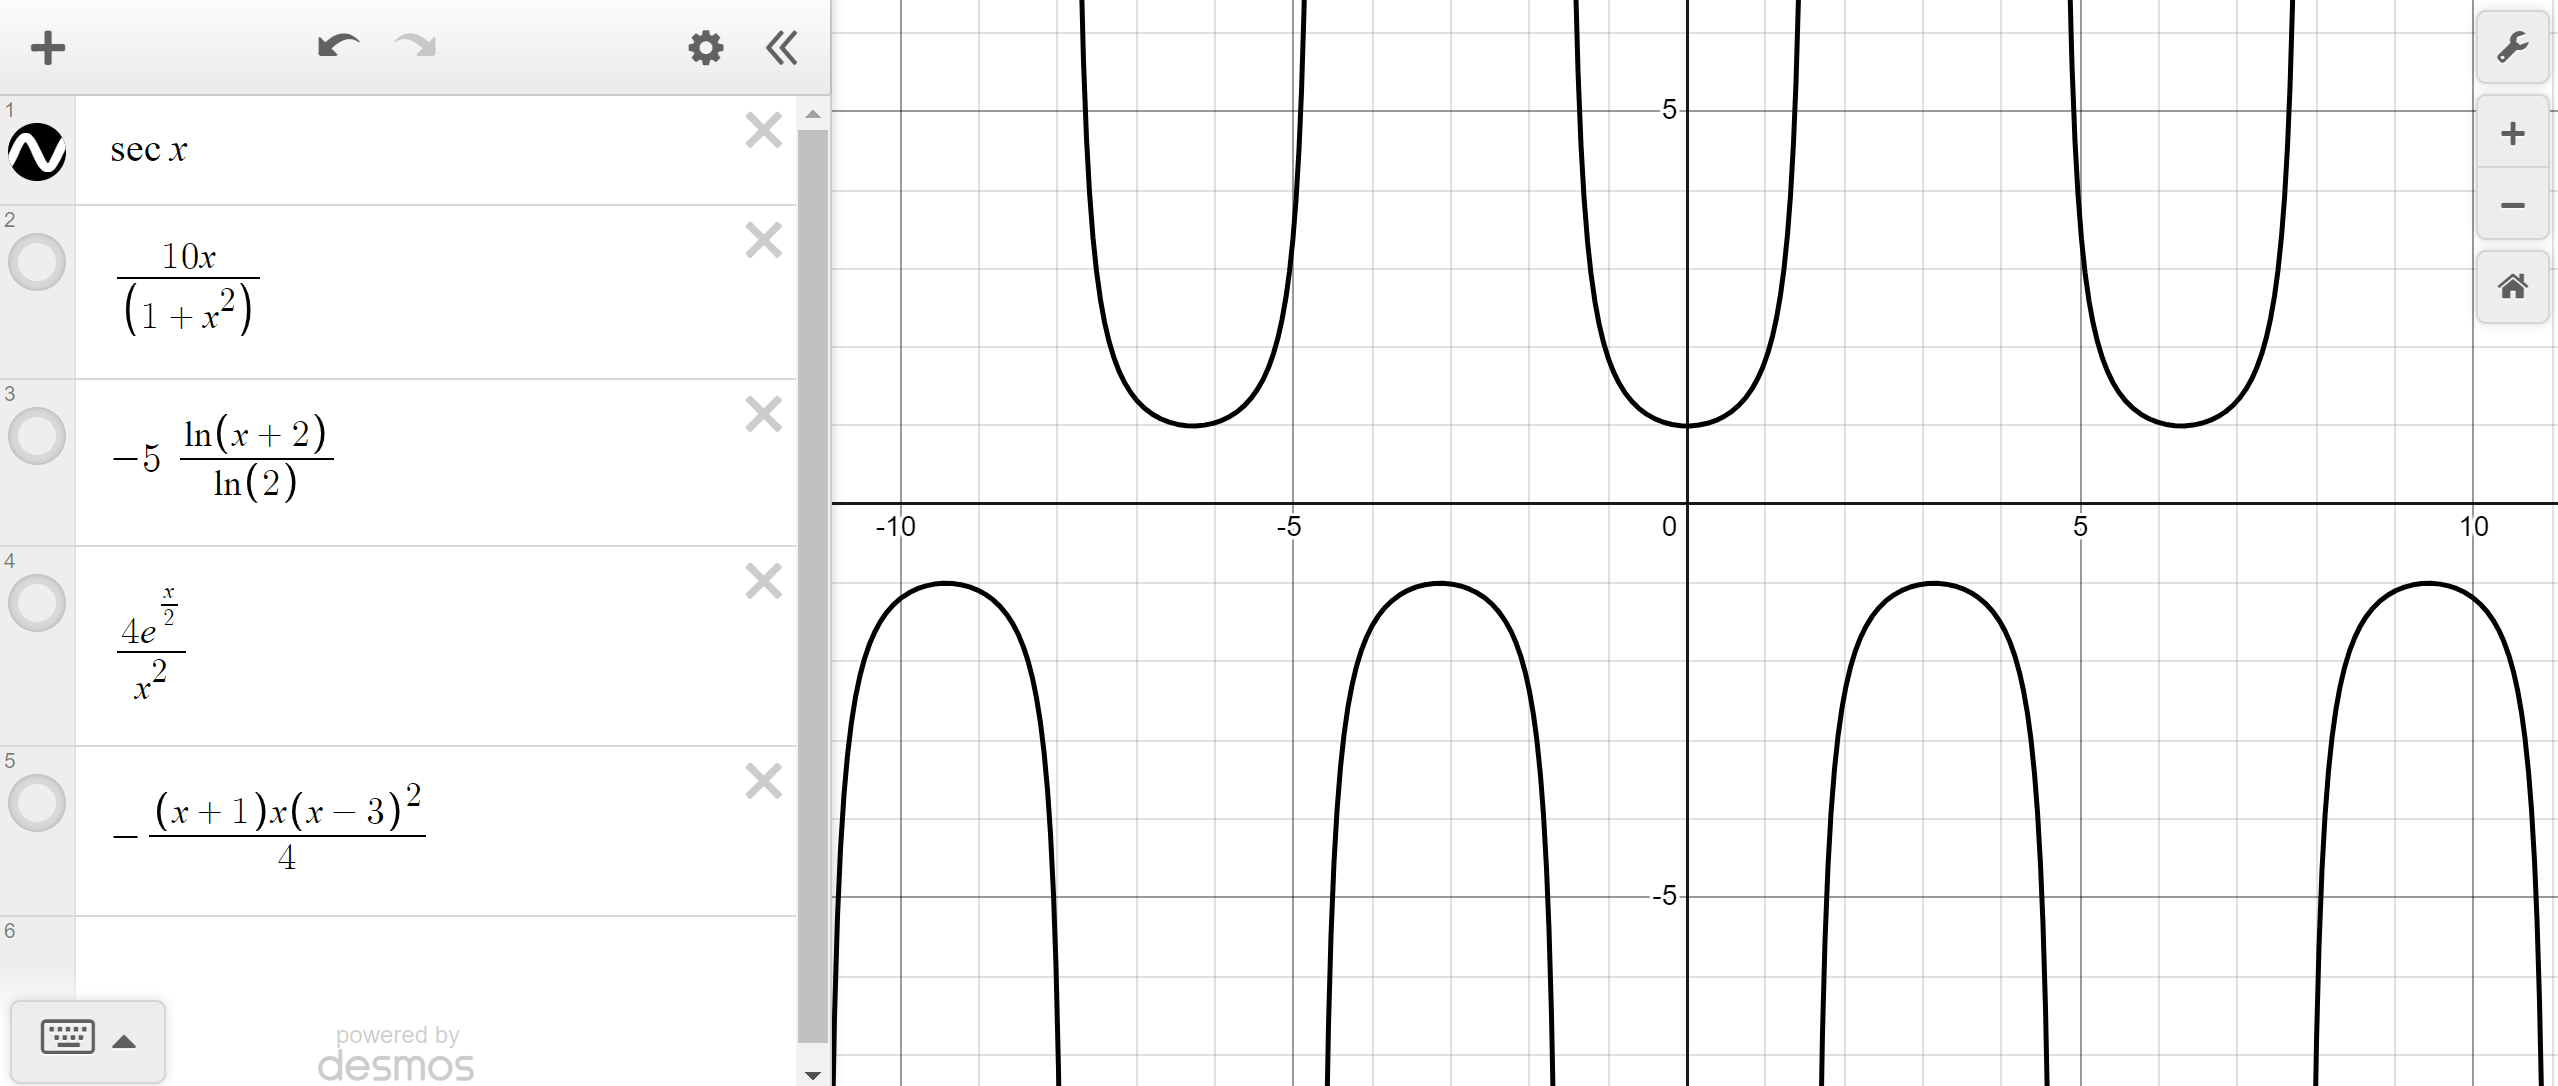
\includegraphics[width=0.9\textwidth]{imgs/imgs FSE/sec_x.png}
    \label{fig:image}
\end{figure}

%%%%%%%%%%%%%%%%%%%%%%%%%%%%%%%%%%%%%%%%%%%%%%%%%%%%%
\newpage
\subsection{Graph 2}
% Second Graph
\begin{figure}[h]
    \centering
    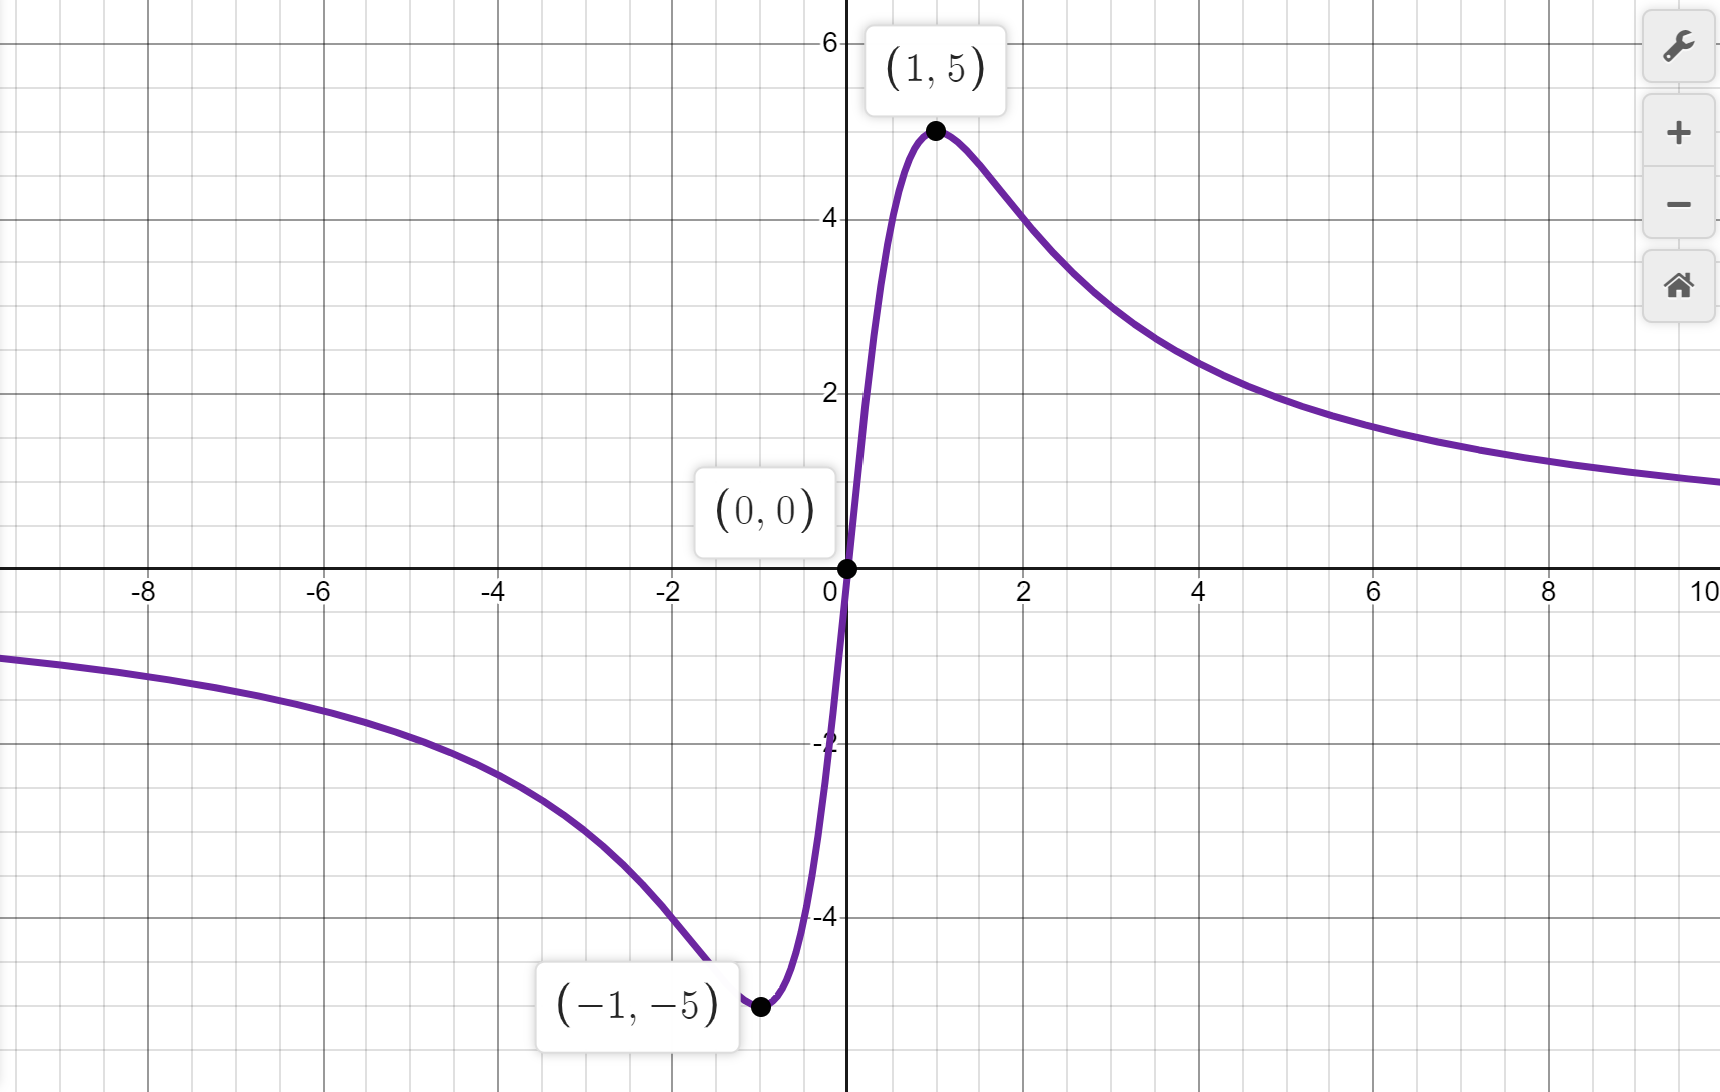
\includegraphics[width=0.9\textwidth]{imgs/imgs FSE/g_2.png}
    \label{fig:image}
\end{figure}

\begin{enumerate}
    \item[a)] \textbf{Key properties:} Rational function with vertical asymptotes at $x = \pm \sqrt{1}$.
    \item[b)]  \textbf{Relationship:} Rational function.
    \item[c)] \textbf{Guess The Equation: } I found my equation for this graph is $$y=\frac{10x}{(1+x^{2})}$$
\end{enumerate}

% Equation of 10/(1+x^2)
\begin{figure}[h]
    \centering
    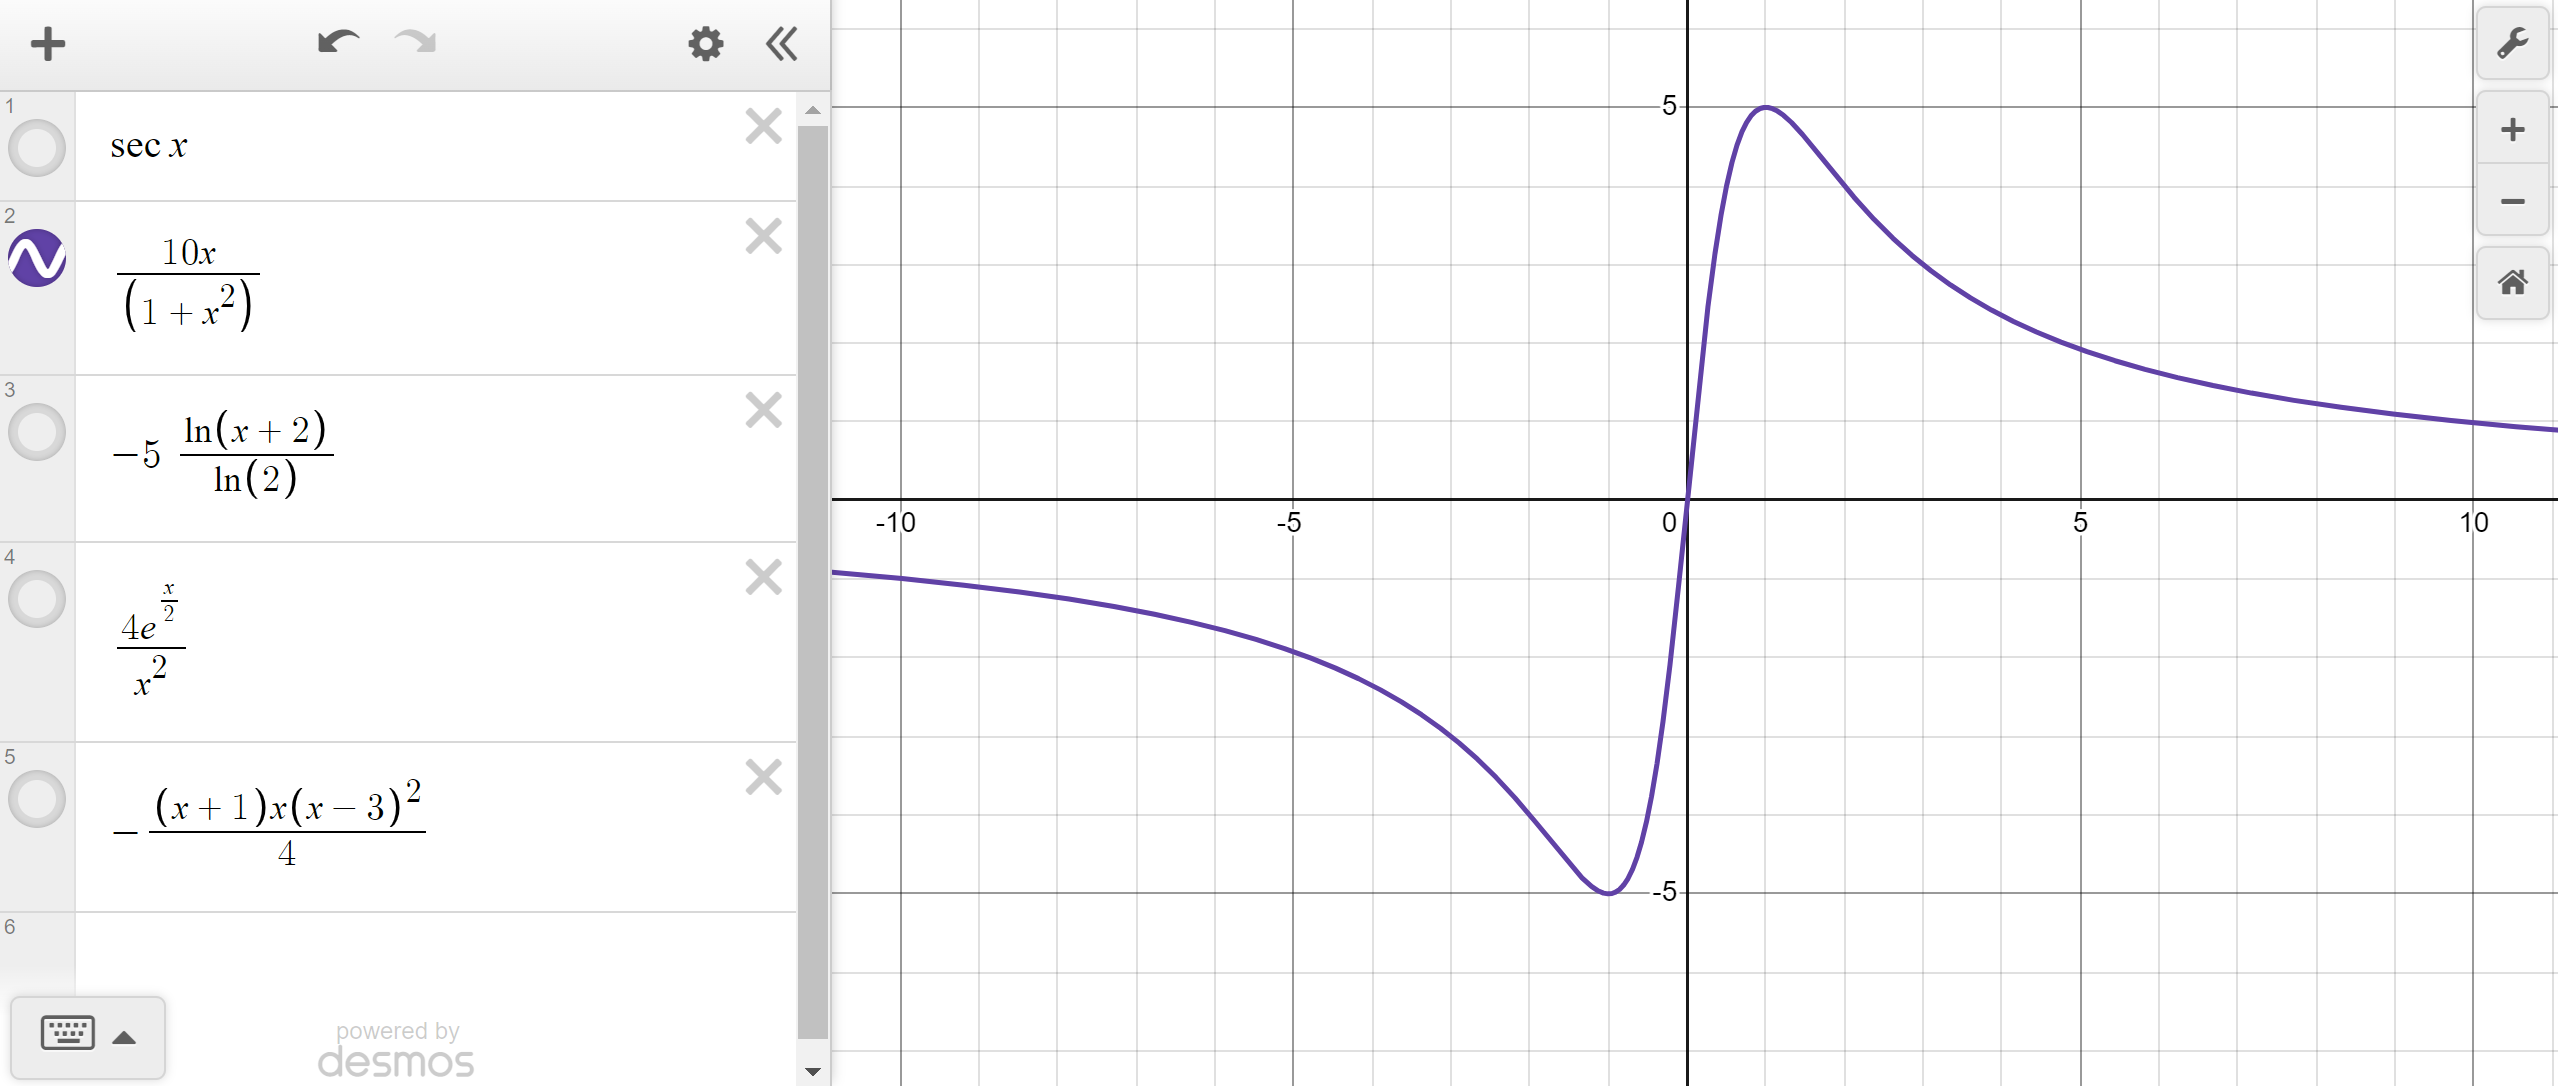
\includegraphics[width=0.9\textwidth]{imgs/imgs FSE/10x_(1+x^2).png}
    \label{fig:image}
\end{figure}
%%%%%%%%%%%%%%%%%%%%%%%%%%%%%%%%%%%%%%%%%%%%%%%%%%%%&
\newpage 

\subsection{Graph 3}
% Third Graph
\begin{figure}[h]
    \centering
    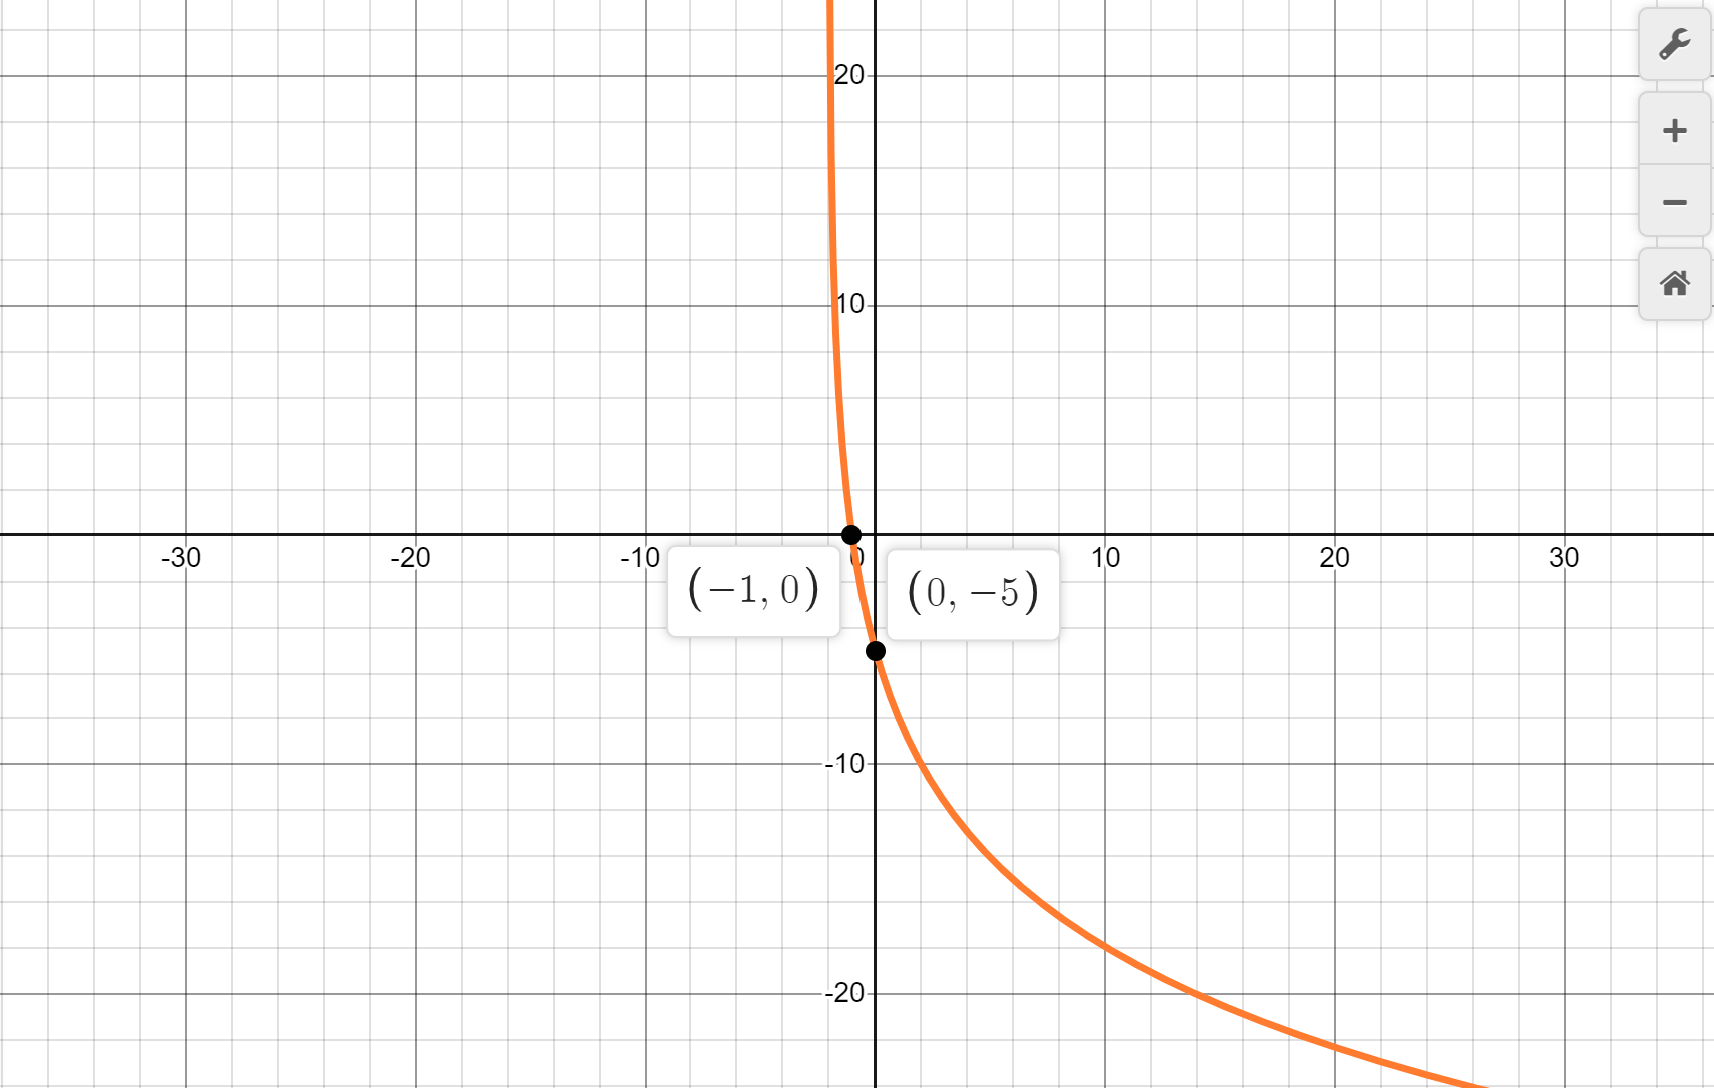
\includegraphics[width=0.9\textwidth]{imgs/imgs FSE/g_3.png}
    \label{fig:image}
\end{figure}
\begin{enumerate}
    \item[a)] \textbf{Key properties:} Logarithmic function with domain $x > -2$.
    \item[b)]  \textbf{Relationship:} Logarithmic function.
    \item[c)] \textbf{Guess The Equation: } I found my equation for this graph is $$y=-5\ \frac{\ln\left(x+2\right)}{\ln\left(2\right)}$$
\end{enumerate}
% Equation of -5ln(x+2)/ln(2)
\begin{figure}[h]
    \centering
    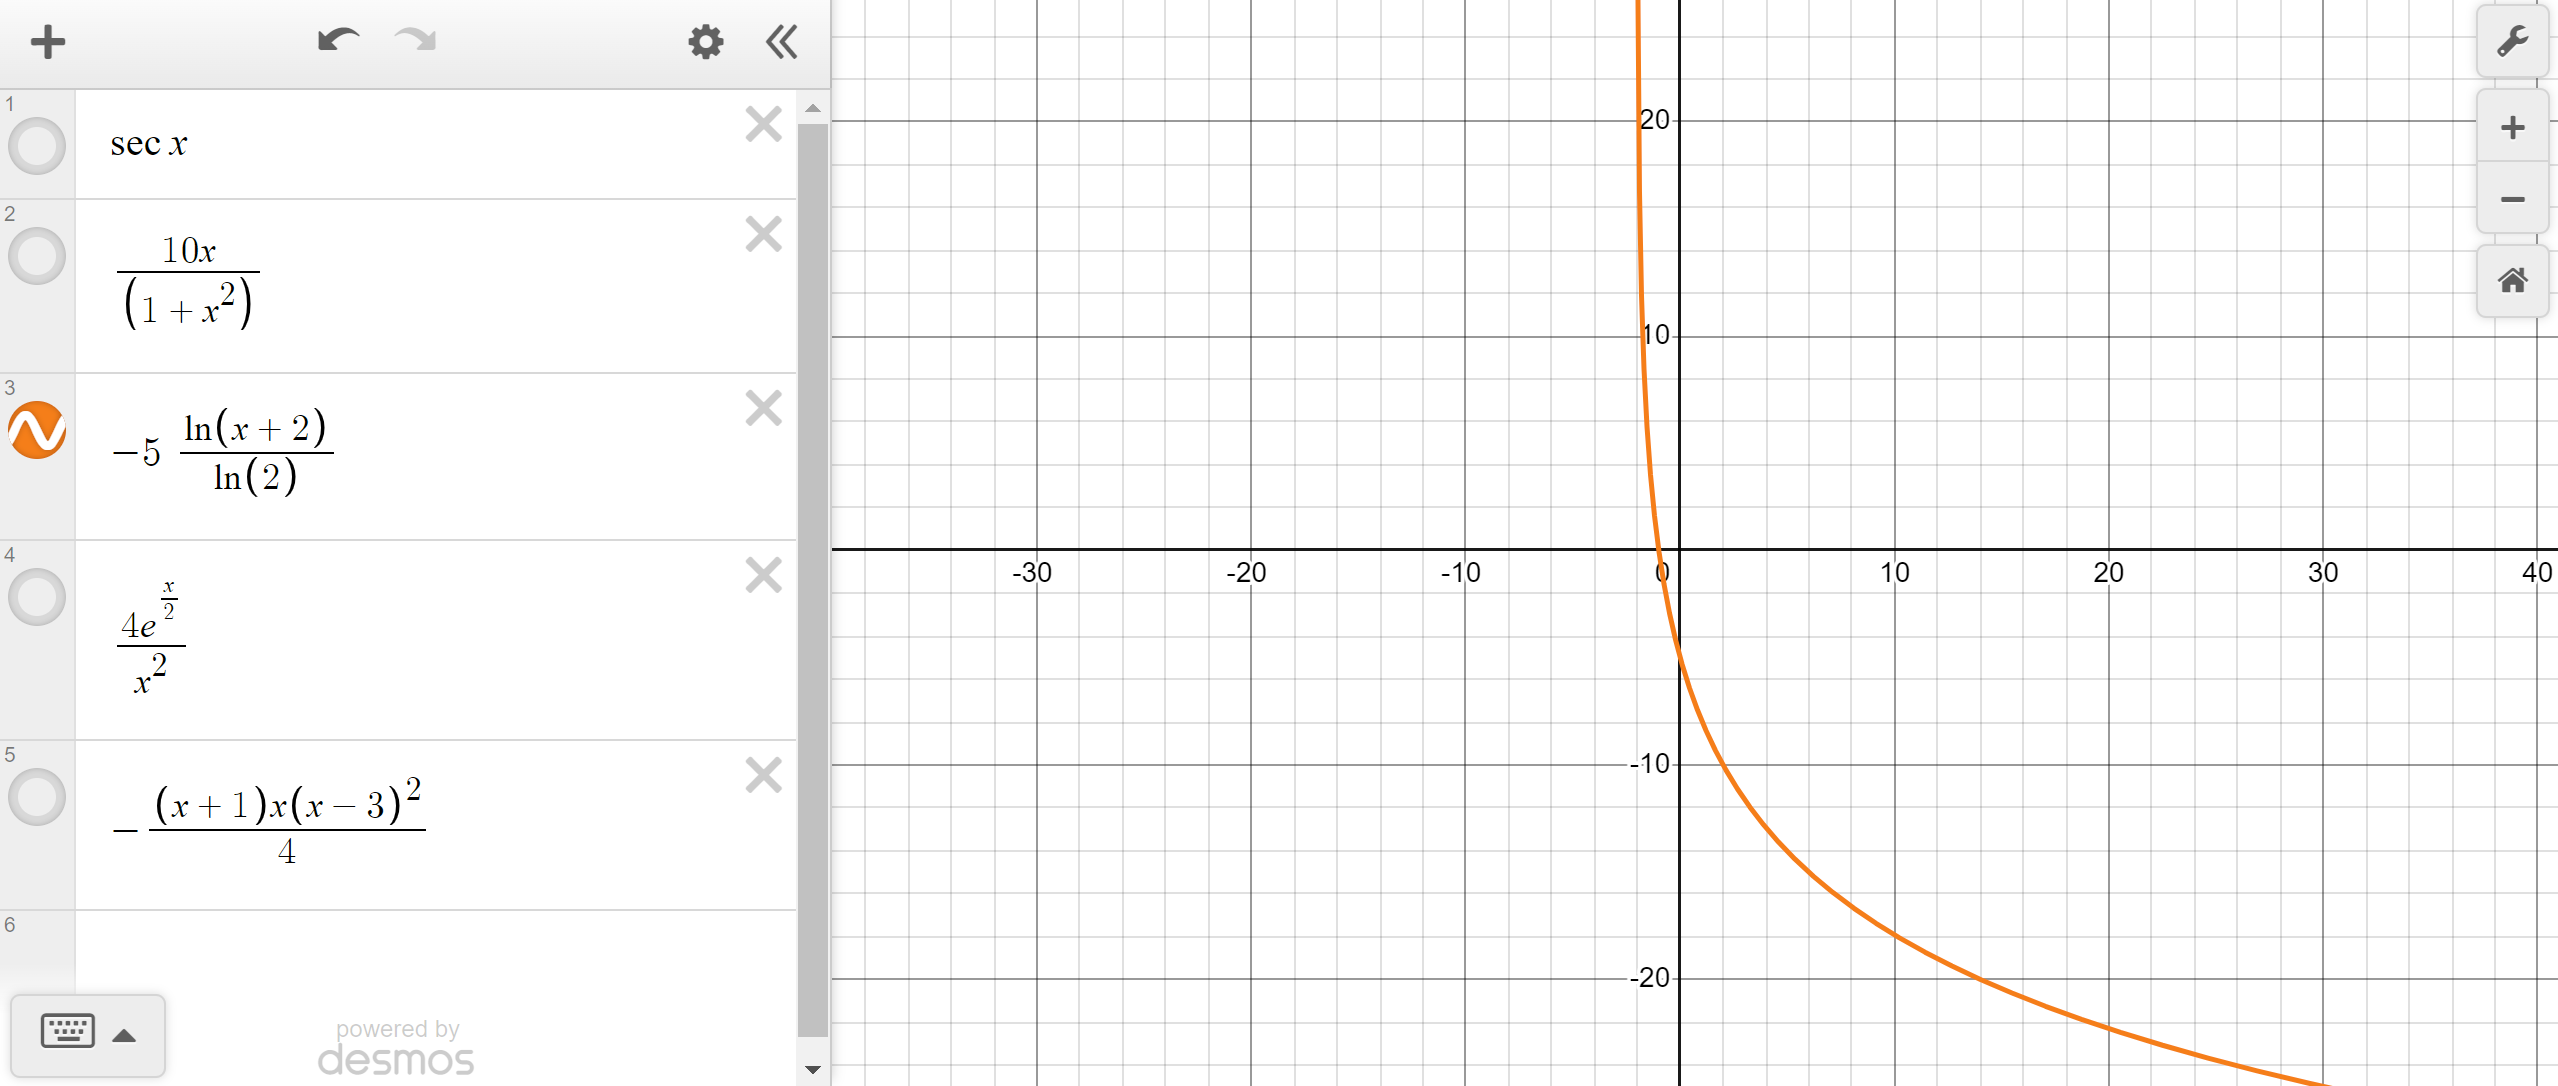
\includegraphics[width=0.9\textwidth]{imgs/imgs FSE/-5_ln(x+2)_ln(2).png}
    \label{fig:image}
\end{figure}
%%%%%%%%%%%%%%%%%%%%%%%%%%%%%%%%%%%%%%%%%%%%%%%%%%%%%
\newpage 

\subsection{Graph 4}
% Fourth Graph
\begin{figure}[h]
    \centering
    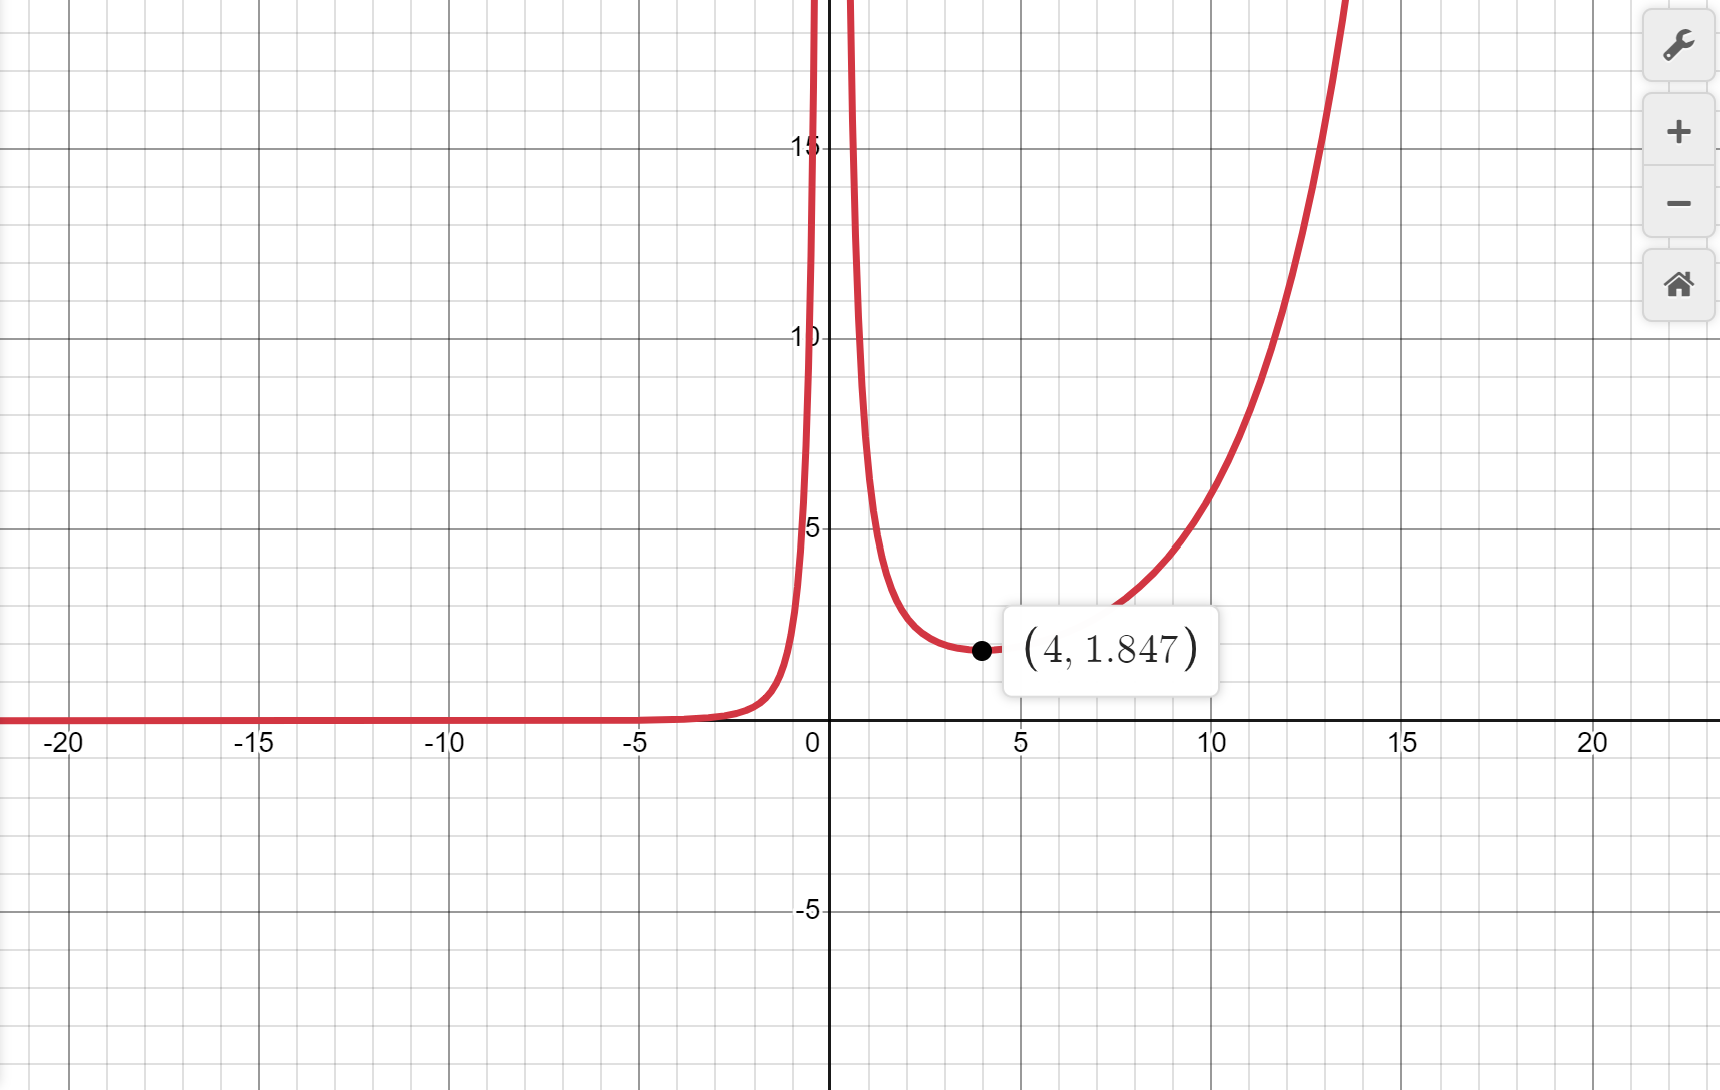
\includegraphics[width=0.9\textwidth]{imgs/imgs FSE/g_4.png}
    \label{fig:image}
\end{figure}
\begin{enumerate}
    \item[a)] \textbf{Key properties:} Exponential function with vertical asymptote at $x = 0$.
    \item[b)]  \textbf{Relationship:} Natural exponential function.
    \item[c)] \textbf{Guess The Equation: } I found my equation for this graph using e \smiley{} $$y=\frac{4e^{\frac{x}{2}}}{x^{2}}$$
\end{enumerate}
% Equation of 4e^x/2 / x^2
\begin{figure}[h]
    \centering
    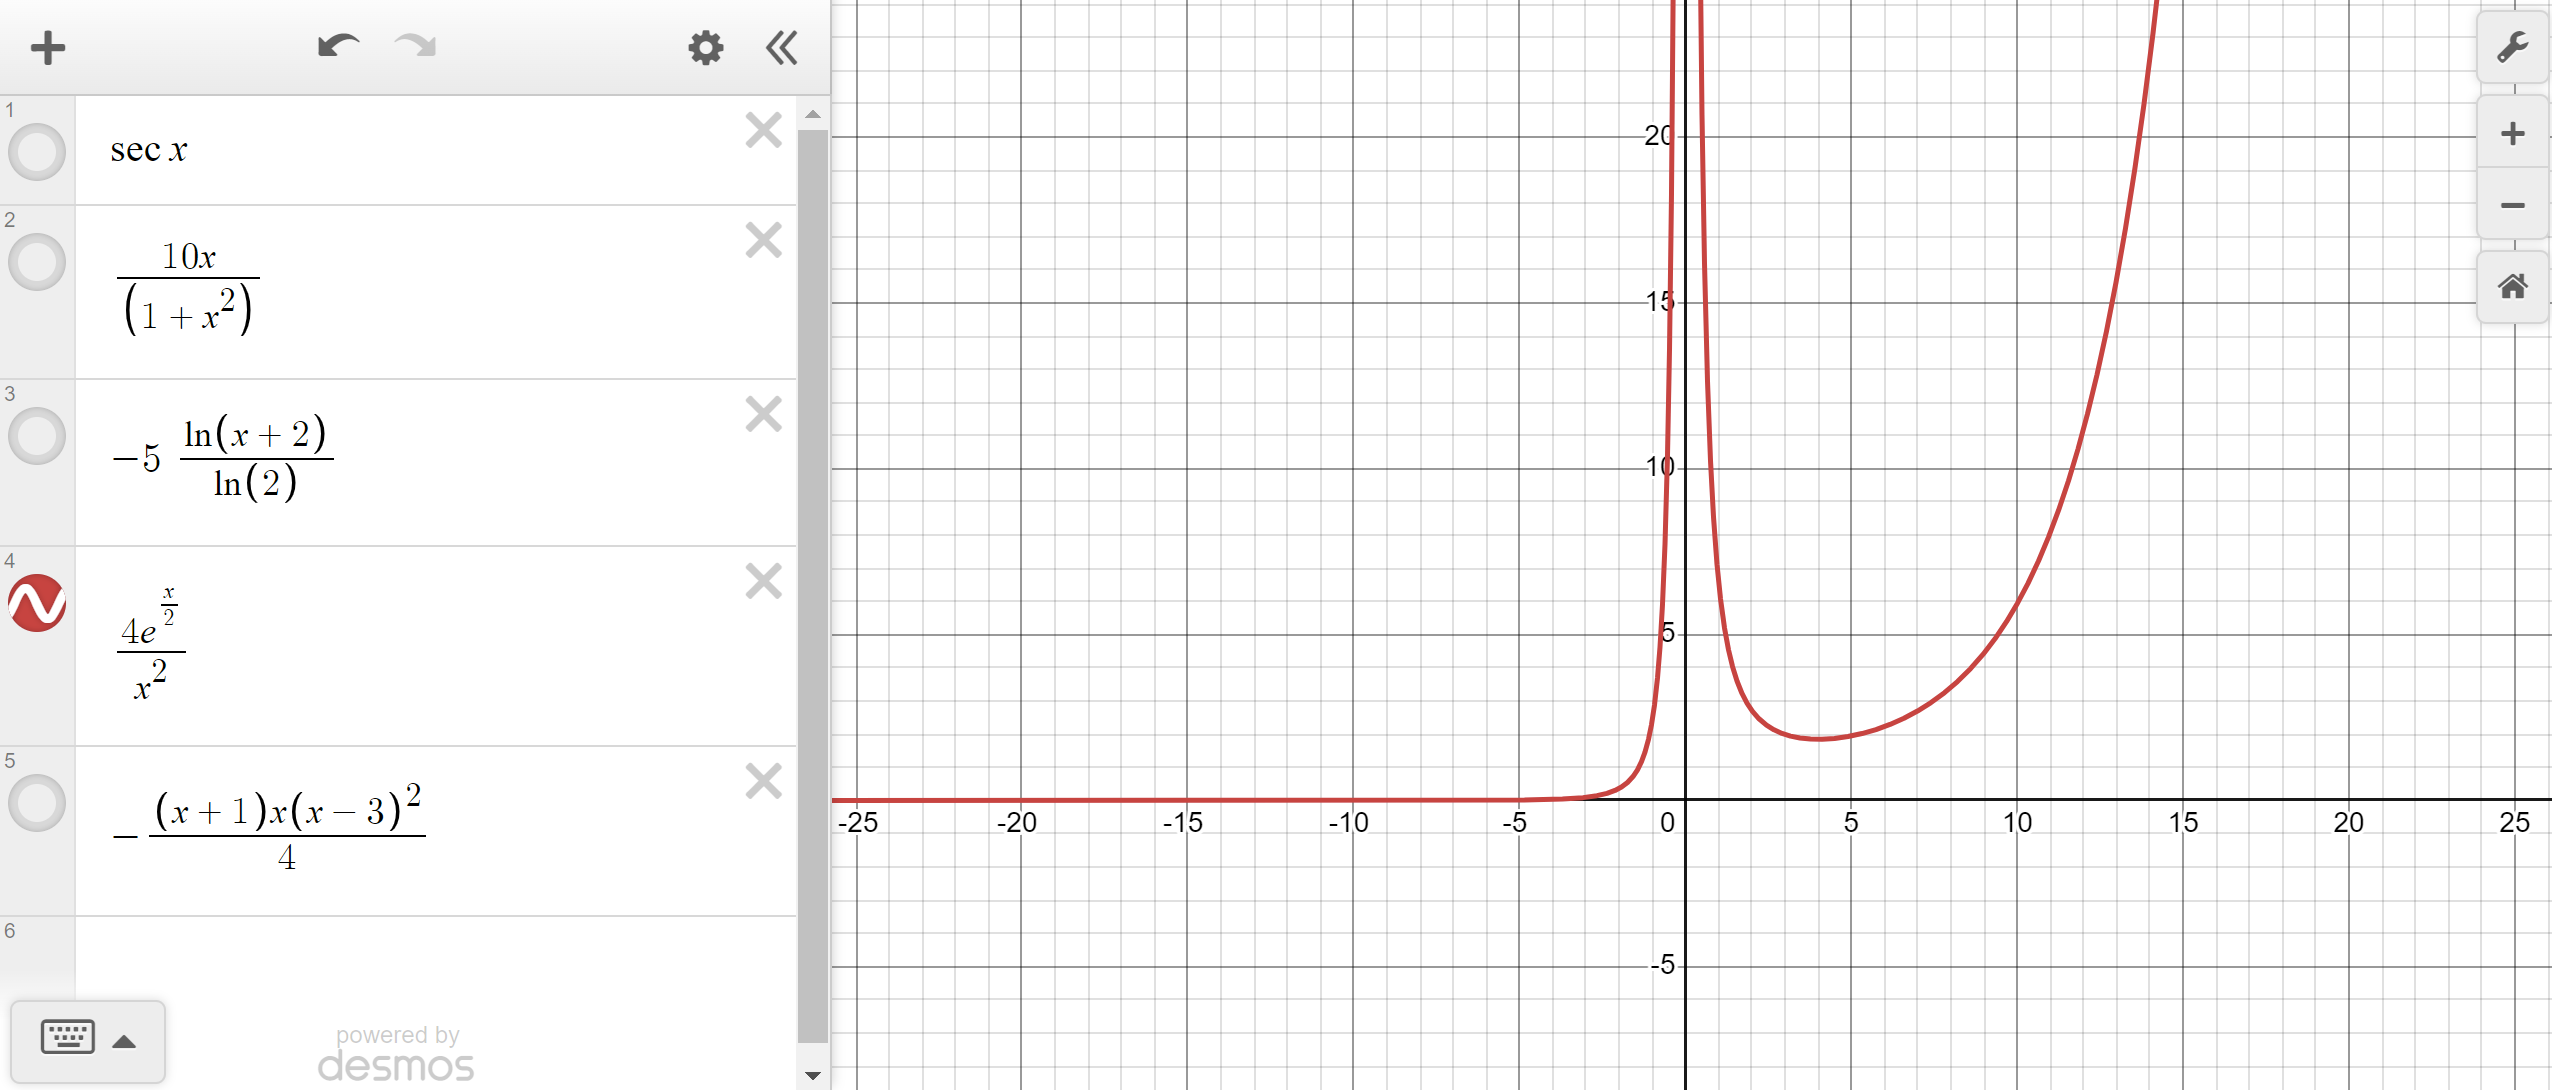
\includegraphics[width=0.9\textwidth]{imgs/imgs FSE/4e^x_2_x^2.png}
    \label{fig:image}
\end{figure}
%%%%%%%%%%%%%%%%%%%%%%%%%%%%%%%%%%%%%%%%%%%%%%%%%%%%%
\newpage 

\subsection{Graph 5}
% Fifth Graph
\begin{figure}[h]
    \centering
    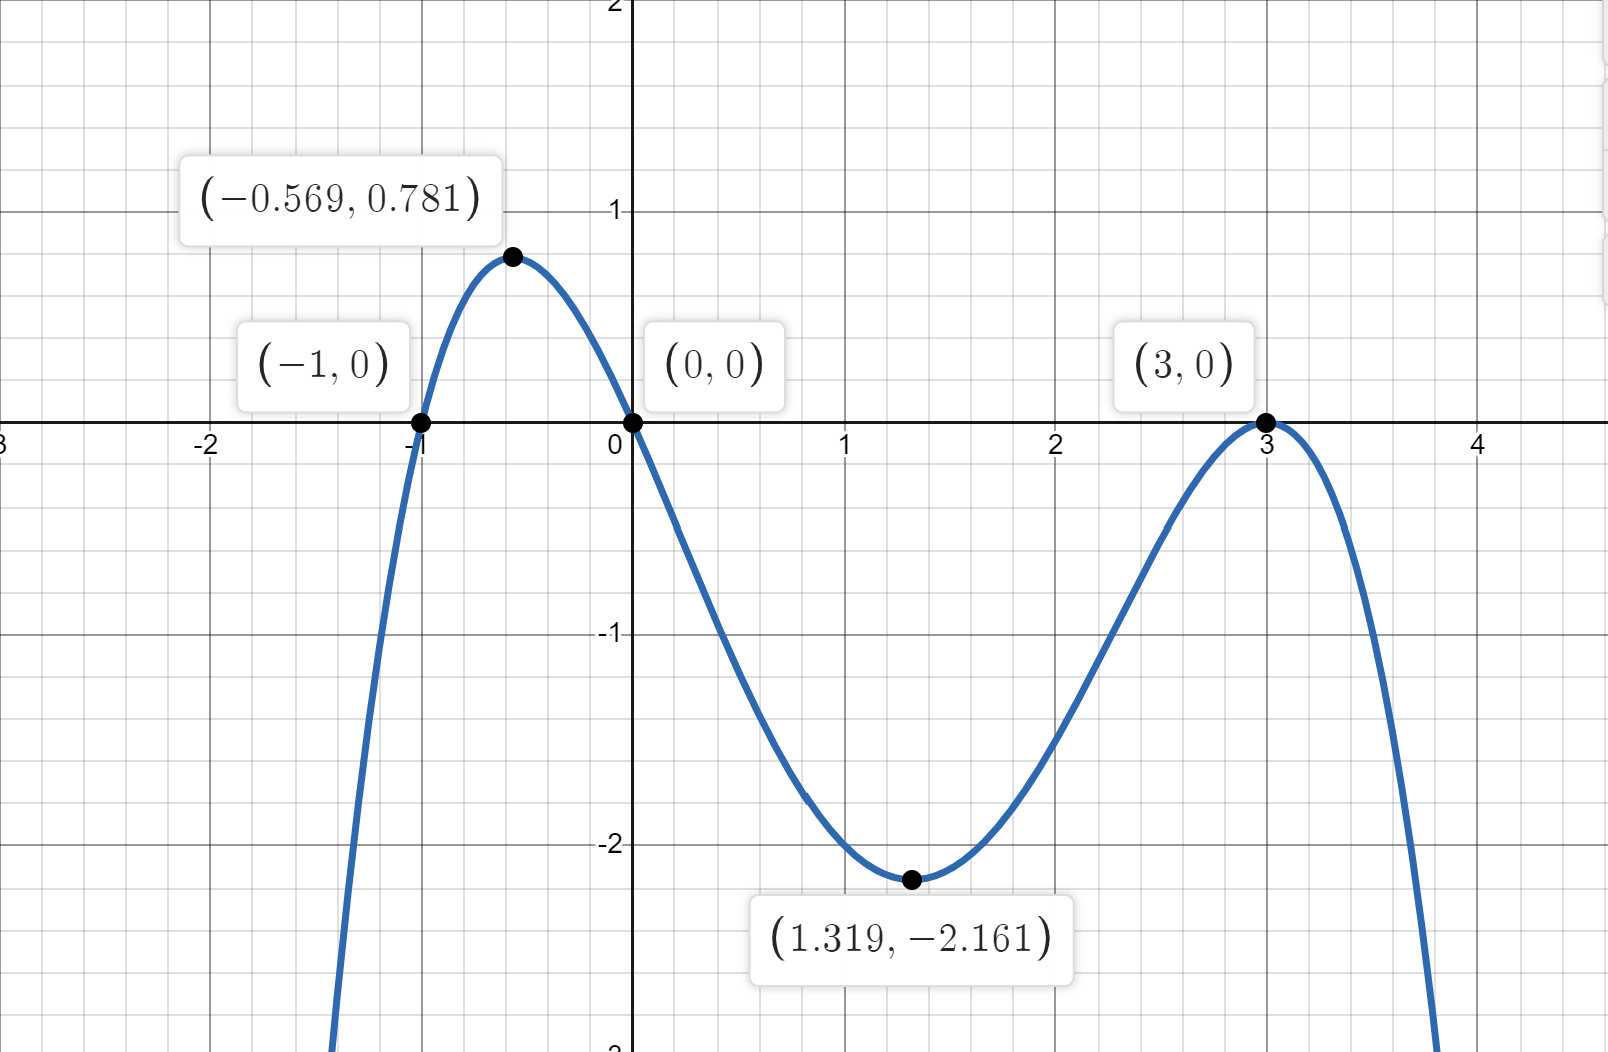
\includegraphics[width=0.9\textwidth]{imgs/imgs FSE/g_5.png}
    \label{fig:image}
\end{figure}
\begin{enumerate}
    \item[a)] \textbf{Key properties:} Polynomial function with roots at $x = -1$ and $x = 3$.
    \item[b)]  \textbf{Relationship:} Polynomial function.
    \item[c)] \textbf{Guess The Equation: } I found my equation for this graph using e :) $$y=-\frac{\left(x+1\right)x\left(x-3\right)^{2}}{4}$$
\end{enumerate}

% Equation of -(x+1)x(x-3)^2/4
\begin{figure}[h]
    \centering
    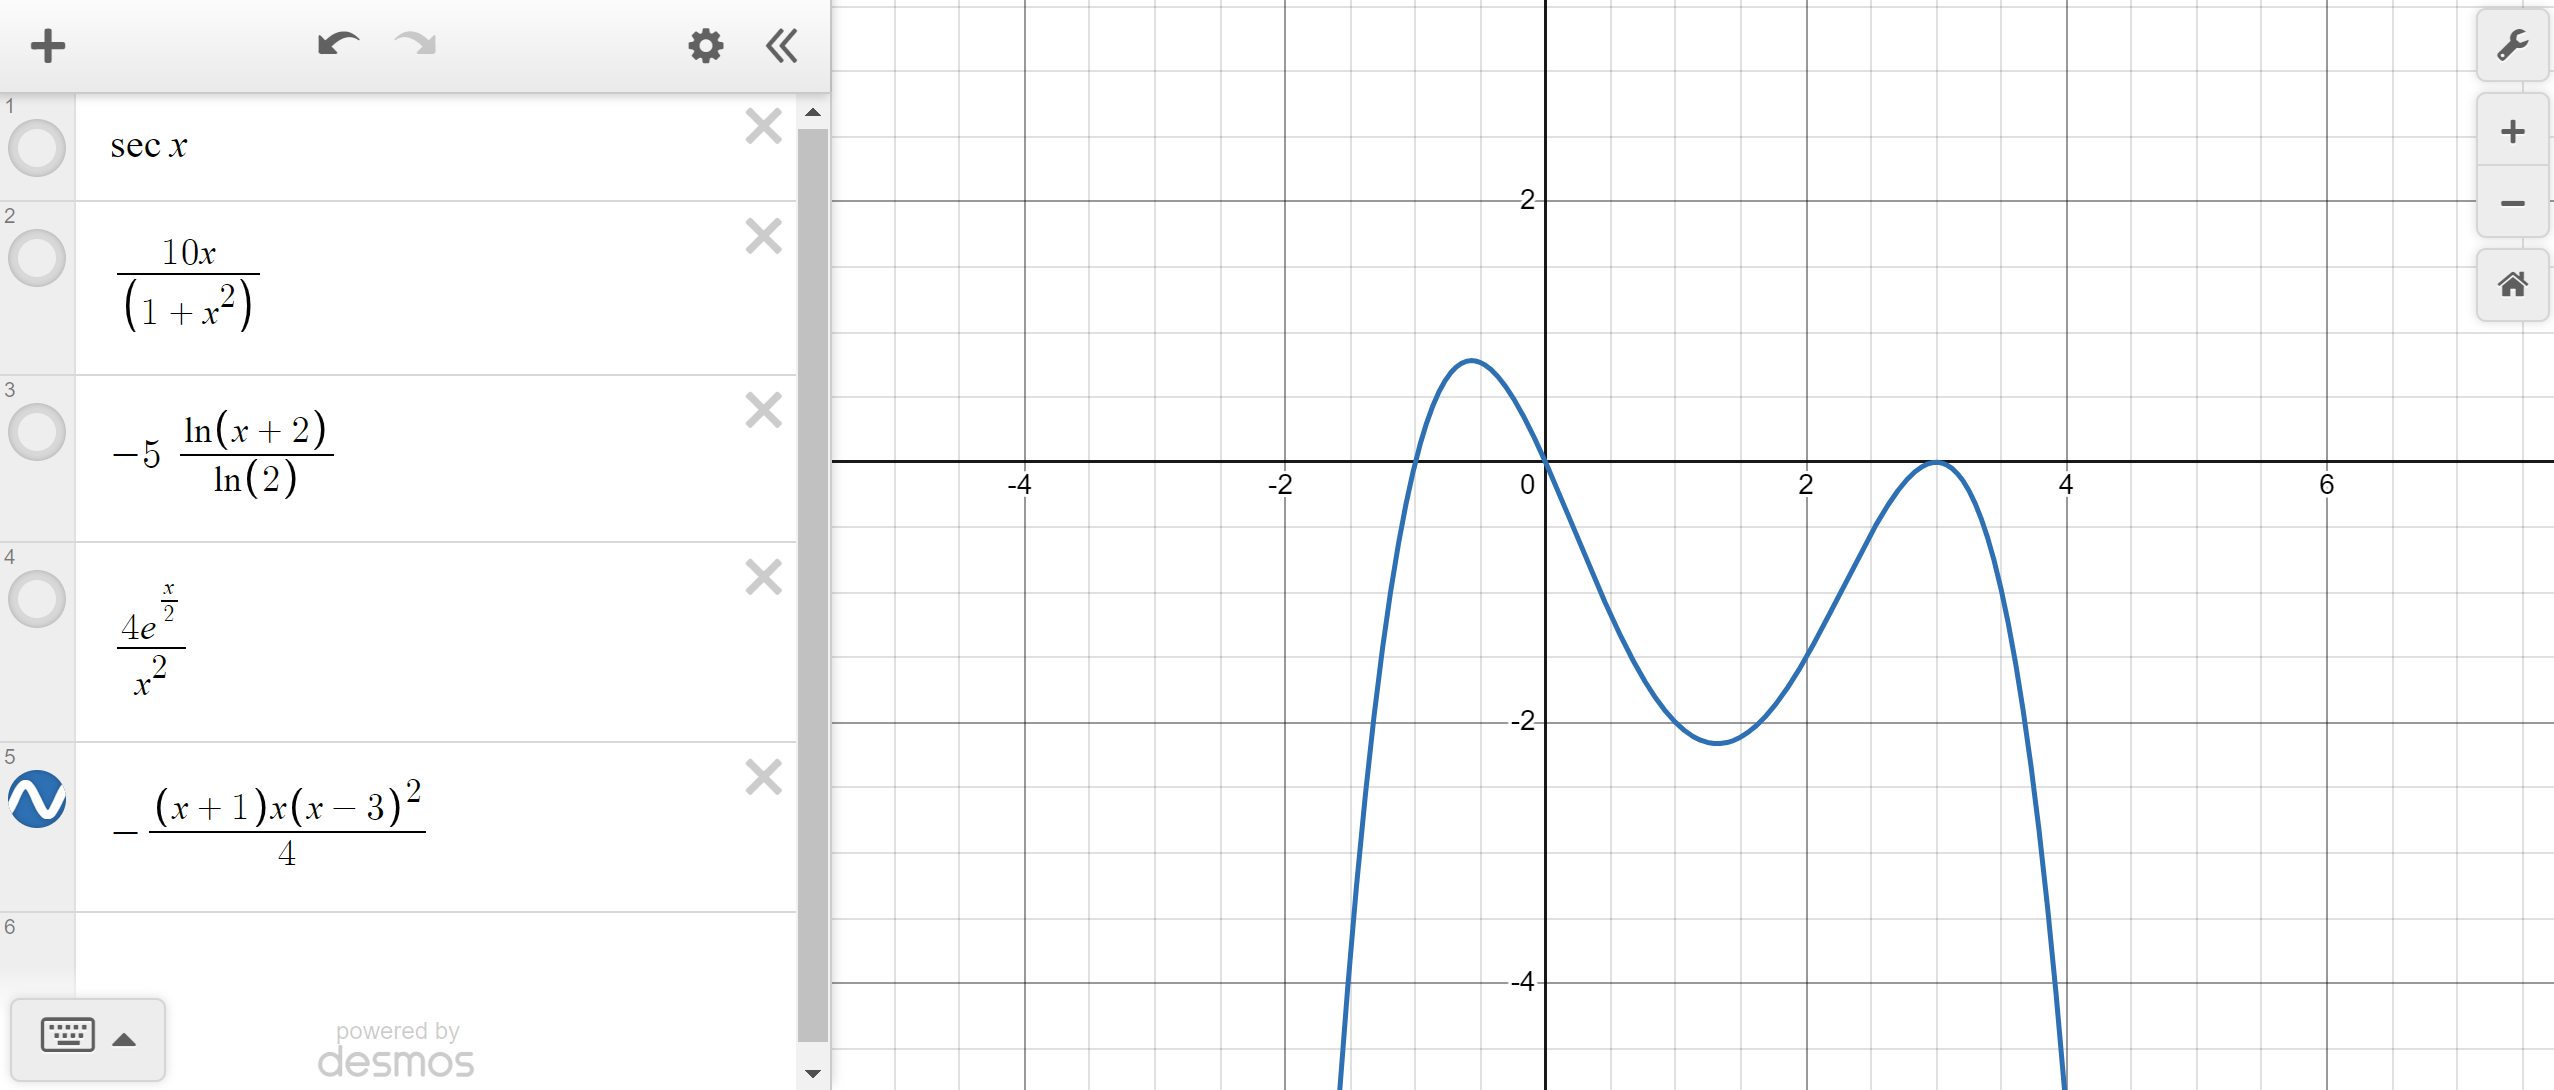
\includegraphics[width=0.9\textwidth]{imgs/imgs FSE/-(x+1)x(x-3)^2_4.png}
    \label{fig:image}
\end{figure}
%%%%%%%%%%%%%%%%%%%%%%%%%%%%%%%%%%%%%%%%%%%%%%%%%%%%%
\newpage

\section*{All equations guessed from graphs are added together at the end.}

% All of Graph
\begin{figure}[h]
    \centering
    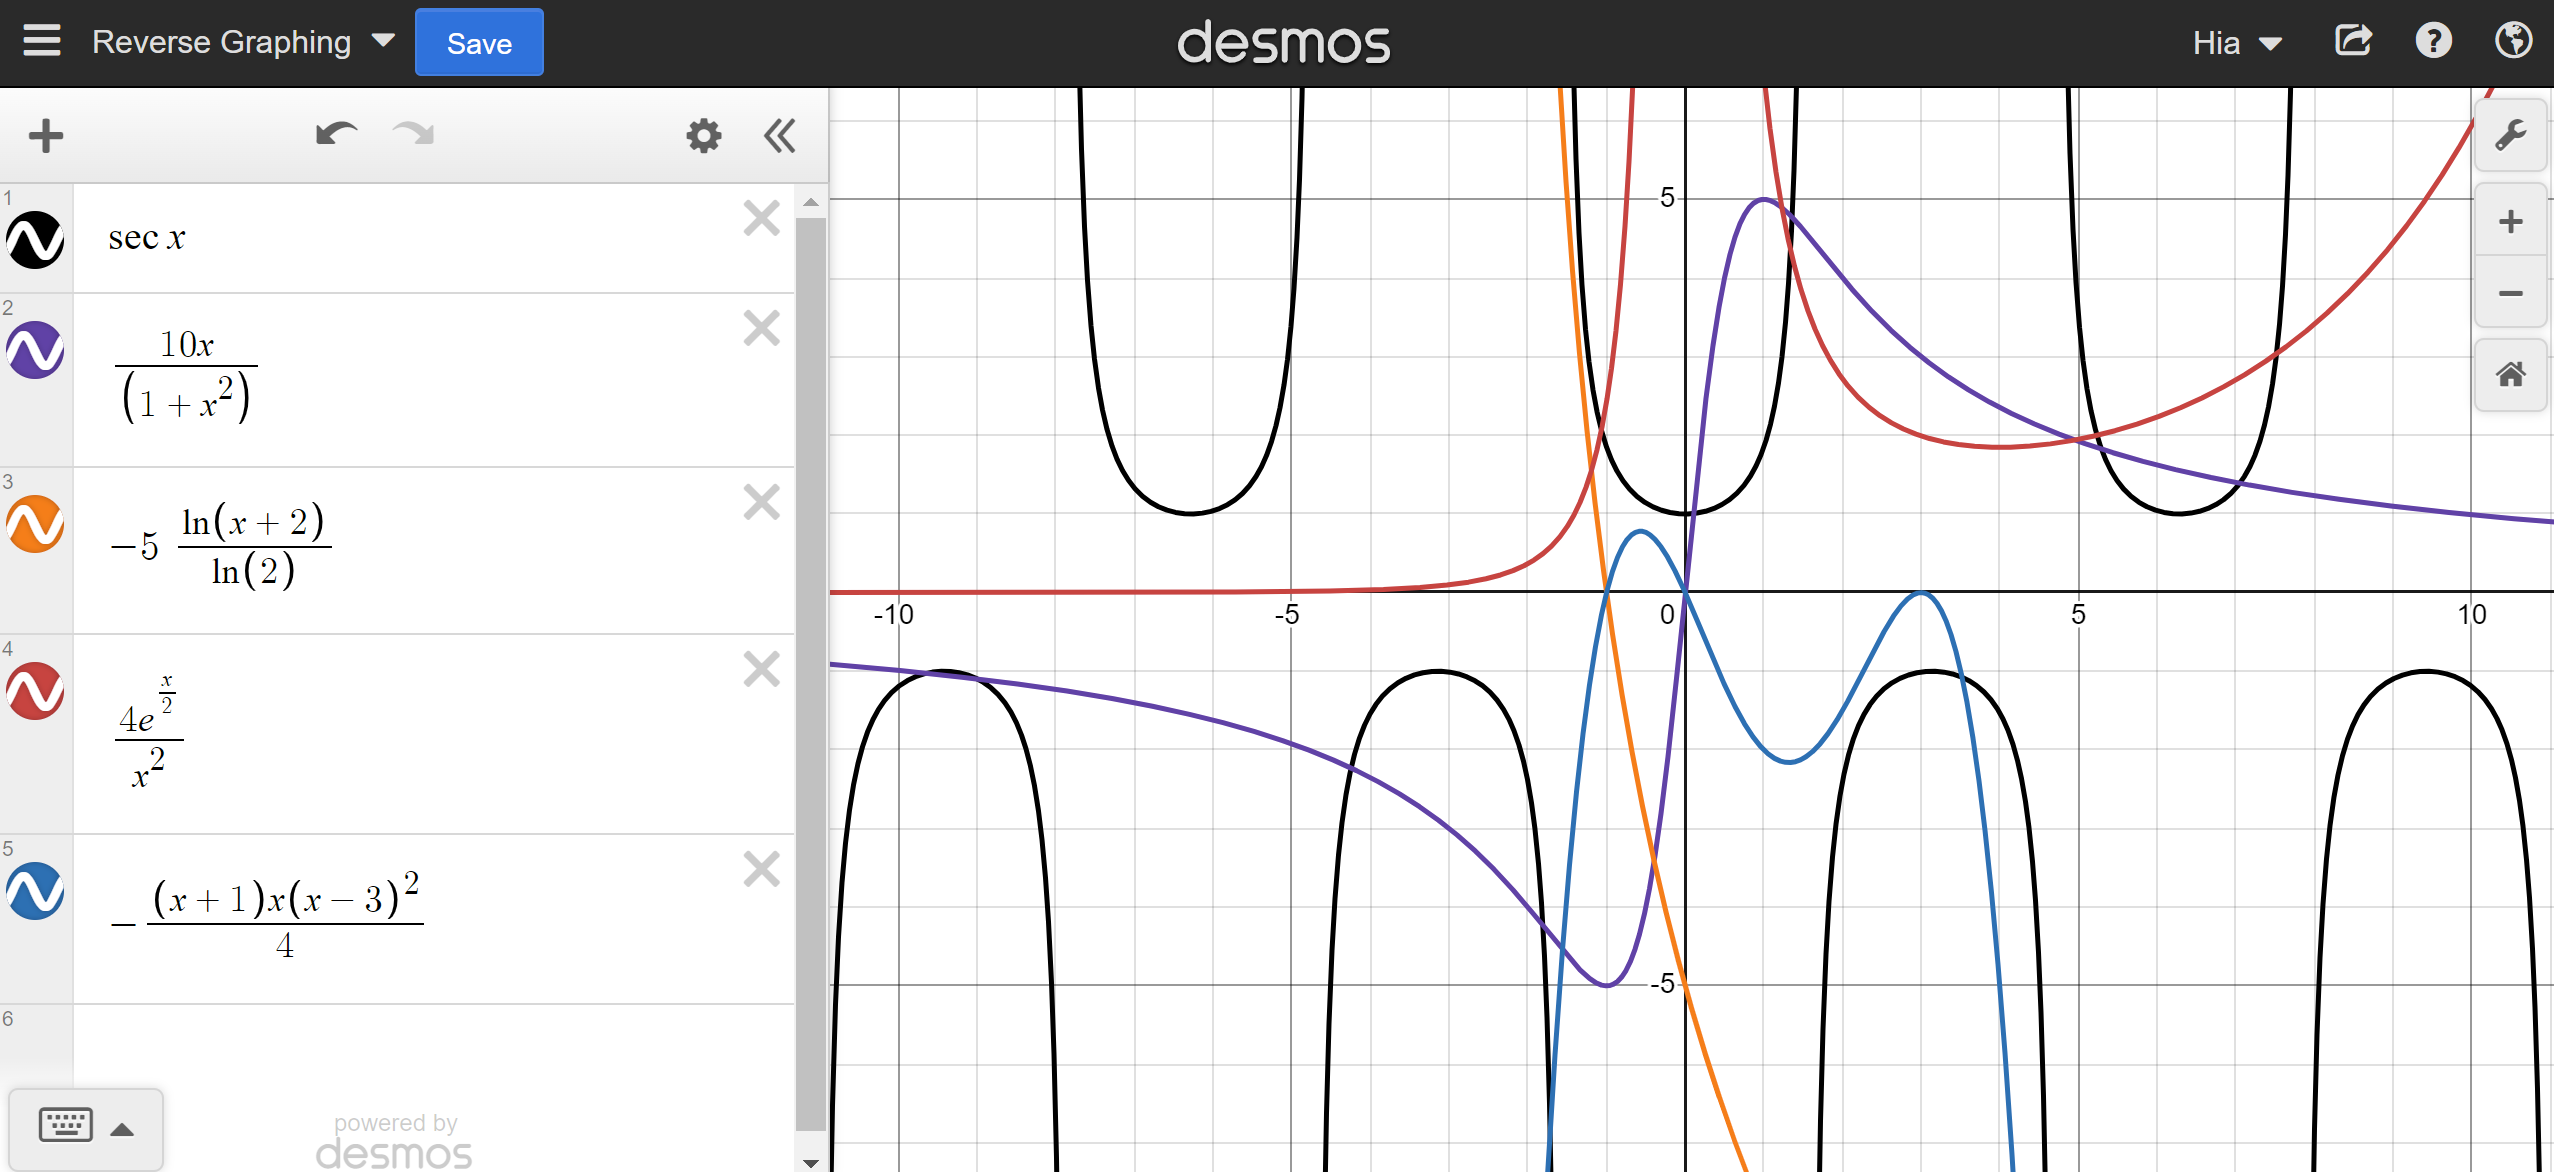
\includegraphics[width=1\textwidth]{imgs/imgs FSE/All_of_them.png}
    \label{fig:image}
\end{figure}
\end{document}